%!TEX root = ../main.tex

\chapter{The background after the LAr veto cut}%
\label{chap:bkg:lar:ph2}

All what has been shown until now concerns data before the LAr and PSD cut. In this
chapter a model of the background after the LAr veto cut will be presented, based on a
Monte Carlo simulation of the LAr scintillation light propagation. Being able to describe
the background after this major event selection is indeed of great interest to study the
distribution of two-neutrino double-beta decay events, which are almost never vetoed by
the LAr veto system. As extensively shown in \cref{chap:theory}, the presence of several
new physics phenomena can be constrained by looking at the shape of the \nnbb\ events
distribution. Understanding the action of the LAr veto cut on background events from the
point of view of the background model requires, however, a full Monte Carlo simulation of
the LAr scintillation mechanism as well as the implementation of all the relevant material
and surface optical properties that contribute to light propagation in the \gerda\ experimental
setup. Implementing such a simulation, as it will be shown, requires an accurate knowledge
of many optical parameters, which is not always the case, unfortunately, with the \gerda\
setup. Nevertheless, it is possible to use special calibration data with low-activity
sources and the LAr veto instrumentation turned on to constrain the LAr veto Monte Carlo
model. An independent analysis of this special data set is used to tune the unknown
optical parameters in the Monte Carlo such to reproduce the observed vetoing performance.
The obtained parameters are then used to produce a map of the LAr scintillation light
detection probability, which is applied to the background model simulations in order to
obtain the LAr veto flag. Based on these new background model pdfs, a statistical analysis
to test possible deviations of the \nnbb\ distribution from its Standard Model description
will be finally presented in the following chapter.
\newpar
The chapter is structured as follows: in \cref{sec:bkg:lar:ph2:data} the data after the
LAr veto cut is presented, sub-divided in the analysis data sets. Then, the development of
the Monte Carlo simulation of the LAr veto system into the \mage\ framework is outlined in
\cref{sec:bkg:lar:ph2:pdfs}. It will be shown how special calibration data is used to tune
the simulation model and how the LAr veto flag for synthetic events is evaluated through a
scintillation light detection probability map. Finally, the background decomposition of
the full-range \gerda\ energy spectrum after the LAr veto cut (\gexpophasetwobkg\ from the
first part of \phasetwo) is presented in \cref{sec:bkg:lar:ph2:gmodel} and discussed in
\cref{sec:bkg:lar:ph2:discussion}.

\section{Analysis data sets}%
\label{sec:bkg:lar:ph2:data}

The background model after the LAr veto cut has been developed using data from the first
part of \gerdatwo, as in \cref{chap:bkg:raw:ph2}. Single- and two- detector events that
survive the LAr veto cut (more in \cref{sec:gerda:cuts}) have been considered: two data
sets from the first category (\enrBEGeII\ and \enrCoaxII) and a single one for the second
(\enrGeII). The exposures documented in \cref{tab:bkg:raw:ph2:datasets} remain the same.
The reader is referred to \cref{sec:bkg:raw:ph2:data} for further details about how these
data sets are constructed.
\newpar
The event energy distributions of the three data sets before and after the LAr veto cut
are displayed in \cref{fig:bkg:lar:ph2:data-desc}: the sum spectrum of \enrBEGeII\ and
\enrCoaxII\ in the top panel and \enrGeII\ in the bottom panel. \g\ peaks and their
Compton shoulders are largely suppressed (e.g.~80\% of the \kvz\ FEP is cut) with the
exception of \kvn, which is a pure \g\ emission (electron capture) and is less likely to
deposit coincident energy in the LAr. After the cut, the spectrum is mainly composed by
\nnbb\ (the LAr veto survival probability is $>99$\%) and residual \a\ events. The
signal-to-background ratio in the \nnbb-dominated region (from 565~keV to 2000~keV
excluding the potassium \g\ lines) improves by a factor 10, jumping from $\sim$2 to
$\sim$~20. This large background reduction motivates the development of a background model
after the LAr veto cut to study the \nnbb\ event distribution with a significant
sensitivity improvement.

\begin{figure}
  \centering
  \includegraphics[width=\textwidth]{plots/bkg/lar/ph2/data-desc.pdf}
  \caption{%
    The data from the first \gexpophasetwobkg\ of \gerdatwo\ before and after the liquid argon veto
    cut, divided into the three background model data sets: \enrBEGeII, \enrCoaxII\ and
    \enrGeII.
  }\label{fig:bkg:lar:ph2:data-desc}
\end{figure}

\section{Monte Carlo simulations and probability density functions}%
\label{sec:bkg:lar:ph2:pdfs}

The Monte Carlo simulation of the liquid argon veto requires to enable the \geant\ optical physics
simulation routines, which have been disabled for the production of the background model
pdfs before analysis cuts (see \cref{sec:bkg:raw:ph2:pdfs}). The relevant material
optical properties needed to simulate the scintillation of LAr and the propagation of the
photons throughout the whole setup have been implemented into \mage\ and documented in
detail in \cref{sec:apdx:mage-optics}. As reported there, unfortunately, many properties
are uncertain or not known at all, especially in the VUV regime ($\sim$128~nm). This
uncertainty propagates to the LAr veto model and the background pdfs, and is treated as a
systematic uncertainty in the \nnbb\ distribution analysis presented in
\cref{chap:2nbb-ana}.

\subsection{Simulating the LAr veto system}%
\label{sec:bkg:lar:ph2:heatmap}

Simulating optical physics is notoriously a computationally intensive task, as the number
of photons to track is very high. Enabling optical processes in background model
simulations, which already take tens of thousands of CPU hours to complete, is not
feasible. To address the issue, an alternative approach to compute the LAr veto flag for
already existing simulations has been developed, based on the construction of a detection
probability map of scintillation photons in LAr. This object, which is going to be
described in this section, will be also be referred to simply as `heat map' or
`probability map' in the following.
\newpar
The first step to produce the probability map is to run a full photon-tracking simulation
of 128~nm scintillation photons in the whole LAr volume defined in \mage. An isotropic
source of VUV photons homogeneously distributed in a pre-selected LAr volume is simulated.
\mage\ allows to restrict the sampling to the volume occupied by LAr only or its
intersection with a geometric solid (e.g.~a cylinder). The photon initial energy is
sampled from a Gaussian distribution with mean 128~nm and variance 2.929~nm. After being
propagated in the implemented \gerda\ setup by the \geant\ core routines, it may hit a
LAr instrumentation sensitive volume (SiPM channel or PMT channel), whose identification
number is finally written on disk. After collecting a sufficient amount of simulated
events, the simulation output is further processed into the probability map. The
three-dimensional LAr volume implemented in \mage\ is partitioned in small boxes (or voxels),
that define a probability validity region. Events generated in a voxel are collected and
the ratio between the number of detected photons (at least one fired LAr veto channel)
over the total is computed.
\[
  p_i = \frac{n_i}{N_i} \pm \frac{1}{N_1}\sqrt{n_i \left(1 - \frac{n_i}{N_1} \right)} \;.
\]
where $n_i$ and $N_i$ are the total number of detected and simulated photons in voxel $i$,
respectively. The binomial uncertainty estimate assumes $N_i>0$ and $n_i<N_i$, which is
always the case for the voxel size considered in this study.  These probability estimates
are saved in a three-dimensional histogram, or LAr light detection probability map. The
\gerda\ Monte Carlo LAr model is thus effectively condensed in this object.
\newpar
The last step is to fold the probability map into the usual background model simulations,
for which no information derived from optical processes is available. Information about
energy depositions by \g, \b\ and \a\ particles in LAr is, in fact, available in the
simulation output and provide the starting point to compute the LAr veto flag. For a given
single energy deposition the number of generated scintillation photons $M$ is drawn from a
Poisson distribution with mean equal to the deposited amount of energy times the LAr
scintillation yield times the LAr Fano factor:
\[
  M \sim \operatorname{P}(E \cdot Y \cdot F) \;.
\]
The number of detected photons is then randomly drawn from a binomial distribution with
success probability $p_k$, where $k$ labels the voxel that contains the LAr hit position,
and number of trials equal to $M$:
\[
  m \sim \operatorname{B}(M, p_k) \;.
\]
If $m>0$ the event is flagged as vetoed by the LAr instrumentation.

\blocktitle{the LAr \\ heat map}
A visualization of an example probability map is given in
\cref{fig:bkg:lar:ph2:larmap:tac}, with one-voxel wide transversal and longitudinal
slices. Voxels are colored according to their probability value: darker areas correspond
to regions in which less scintillation photons reach the LAr veto detectors and therefore
the vetoing efficiency is worse. It is worth to let the reader note how the detection
probability reaches very low values in the LAr volume enclosed by germanium detectors, as
photons get easily trapped in such a complex geometry. On the other hand, the closer to
PMTs and fibers the photons are produce, the higher their detection probability. In the
horizontal slice one can also appreciate the effect of the different SiPM channel
efficiencies, which break the rotational invariance of the map.
\begin{figure}
  \centering
  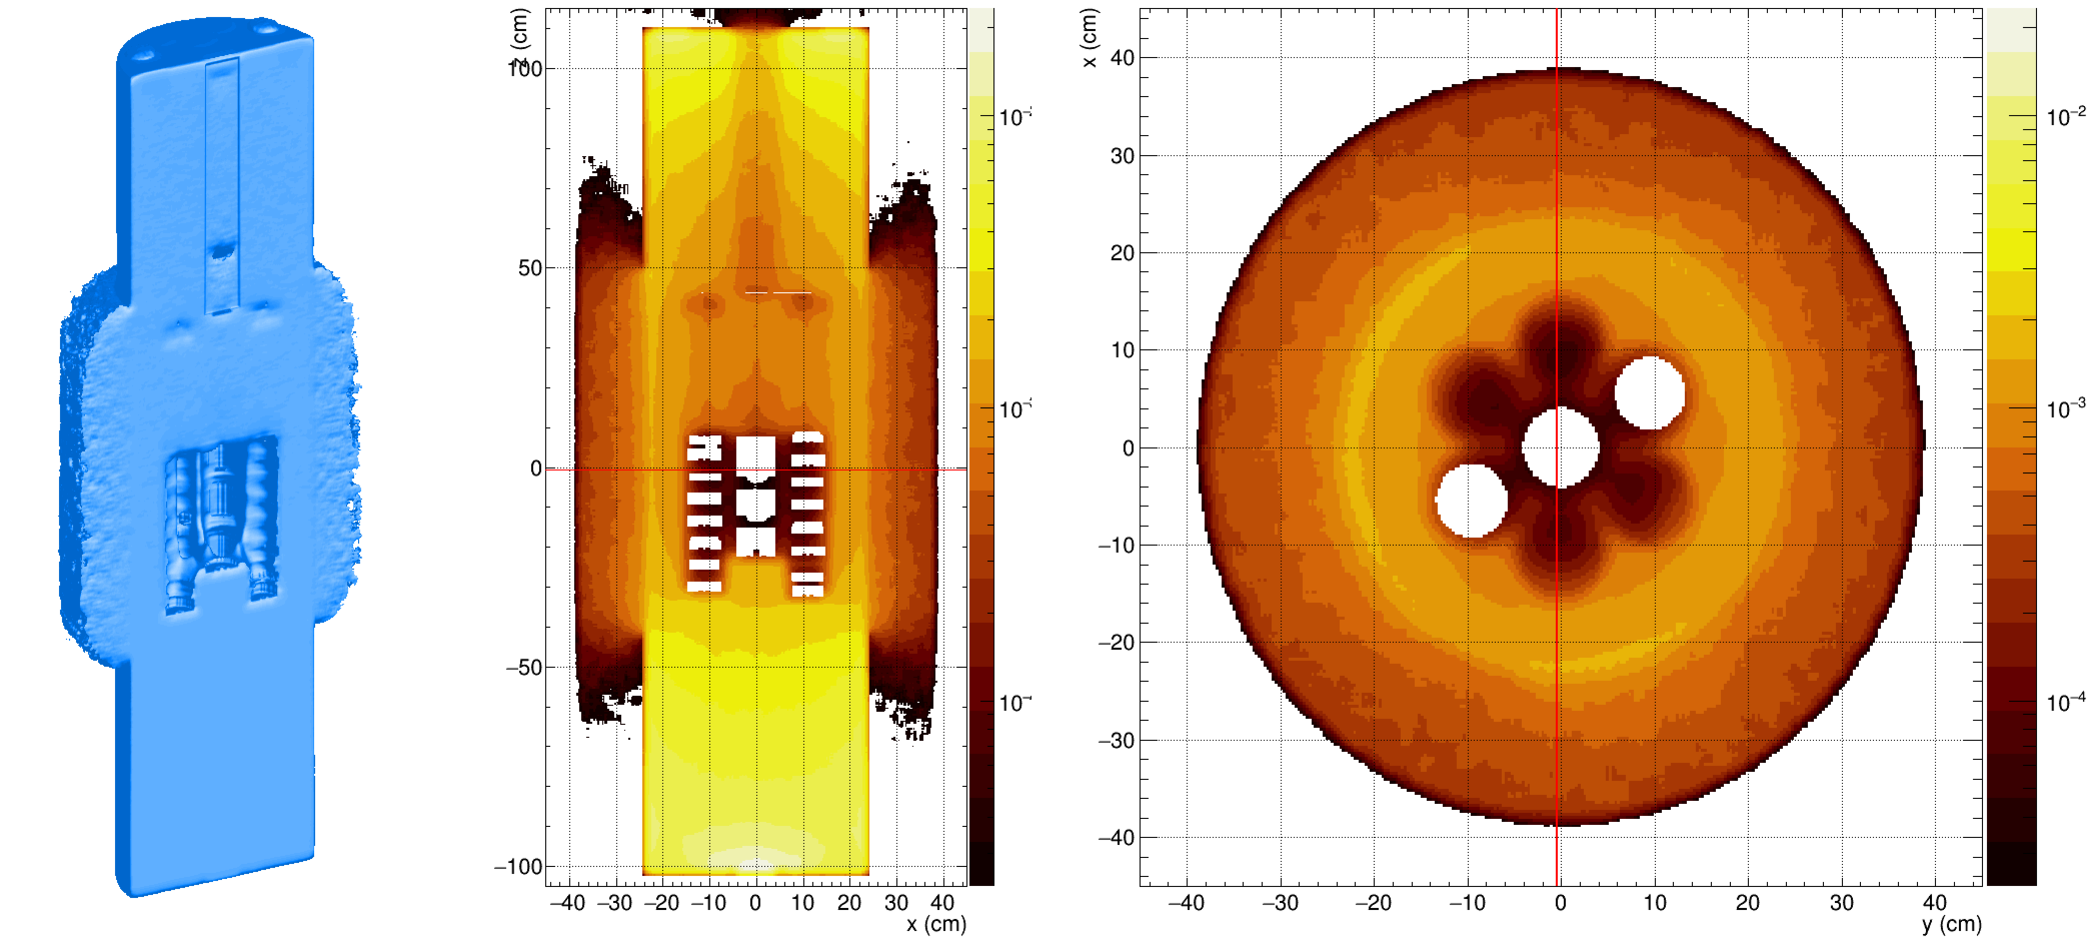
\includegraphics[width=0.9\linewidth]{plots/bkg/lar/ph2/larmodel/larmap-tac.png}
  \caption{%
    The three-dimensional LAr photon detection probability map interactive viewer.
    Two-dimensional longitudinal and transversal sections are displayed in the second and
    third pad from the left corresponding to the user pointer position on the 3D
    rendering in the first pad. Red lines mark the cut positions. A smoothing algorithm is
    applied to wash out statistical fluctuations and make the map look more homogeneous to
    the eye.
  }\label{fig:bkg:lar:ph2:larmap:tac}
\end{figure}
\newpar
As remarked in \cref{sec:bkg:lar:ph2:mage}, uncertainties on the optical specifications
implemented in \mage\ can be quite large. Properties like the LAr scintillation yield and
attenuation length, the germanium reflectivity and the TPB quantum efficiency can possibly
have a large impact on the probability map. Other crucial unknowns are the SiPM and PMT
channel efficiencies and the coverage of the fiber shroud, defined as the fraction of
lateral surface area of the curtain occupied by fiber material. Channel efficiencies
extracted from physics data cannot be used, as the simulated efficiencies account for
various other effects in the Monte Carlo and can therefore be quite different. The fiber
coverage on the other hand should be around 0.5, but there could be shrinking phenomena or
single-fiber twists in LAr which could make the real coverage significantly different.
\newpar
To understand the systematic impact of these parameters on the LAr probability map, a
dedicated Monte Carlo study has been performed. A set of representative voxels has been
selected, whose location is documented in \cref{fig:bkg:lar:ph2:larmap:dist}, rightmost
image. For each of these voxels the probability dependence on some Monte Carlo parameters
has been investigated, giving the results displayed in the remaining plots of
\cref{fig:bkg:lar:ph2:larmap:dist}. Voxels have been considered along the central array
axis (green), just outside (blue) and inside (red) the fiber shroud. Three additional
voxels have been chosen in the low-probability region inside the germanium array (black
and violet). Three properties have been taken into consideration for this study: the
germanium reflectivity, the fiber shroud coverage and the LAr absorption length. The
reflectivity has been scaled with a global factor, such that the unit value refers to the
value implemented in \mage. Two qualitatively different trends can be noticed: the
reflectivity and coverage impact is approximately linear in the considered interval, while
the absorption length acts more exponentially on probabilities. This is compatible with
the assumption that attenuation in matter generally follows an exponential law. However a
partial saturation effect seems to take place after about 40~cm, when the typical photon
free path length in the \gerda\ setup is reached. The impact of a parameter depends on the
voxel location too. As instance, the probability in the black voxel between \GD{89B} and
\GD{02D} changes drastically upon different germanium reflectivity assumptions. On the
other hand, orange and red voxel close to the fibers (where the calibration sources are)
are the most sensitive to modifications of the fiber shroud coverage.

\begin{figure}
  \centering
  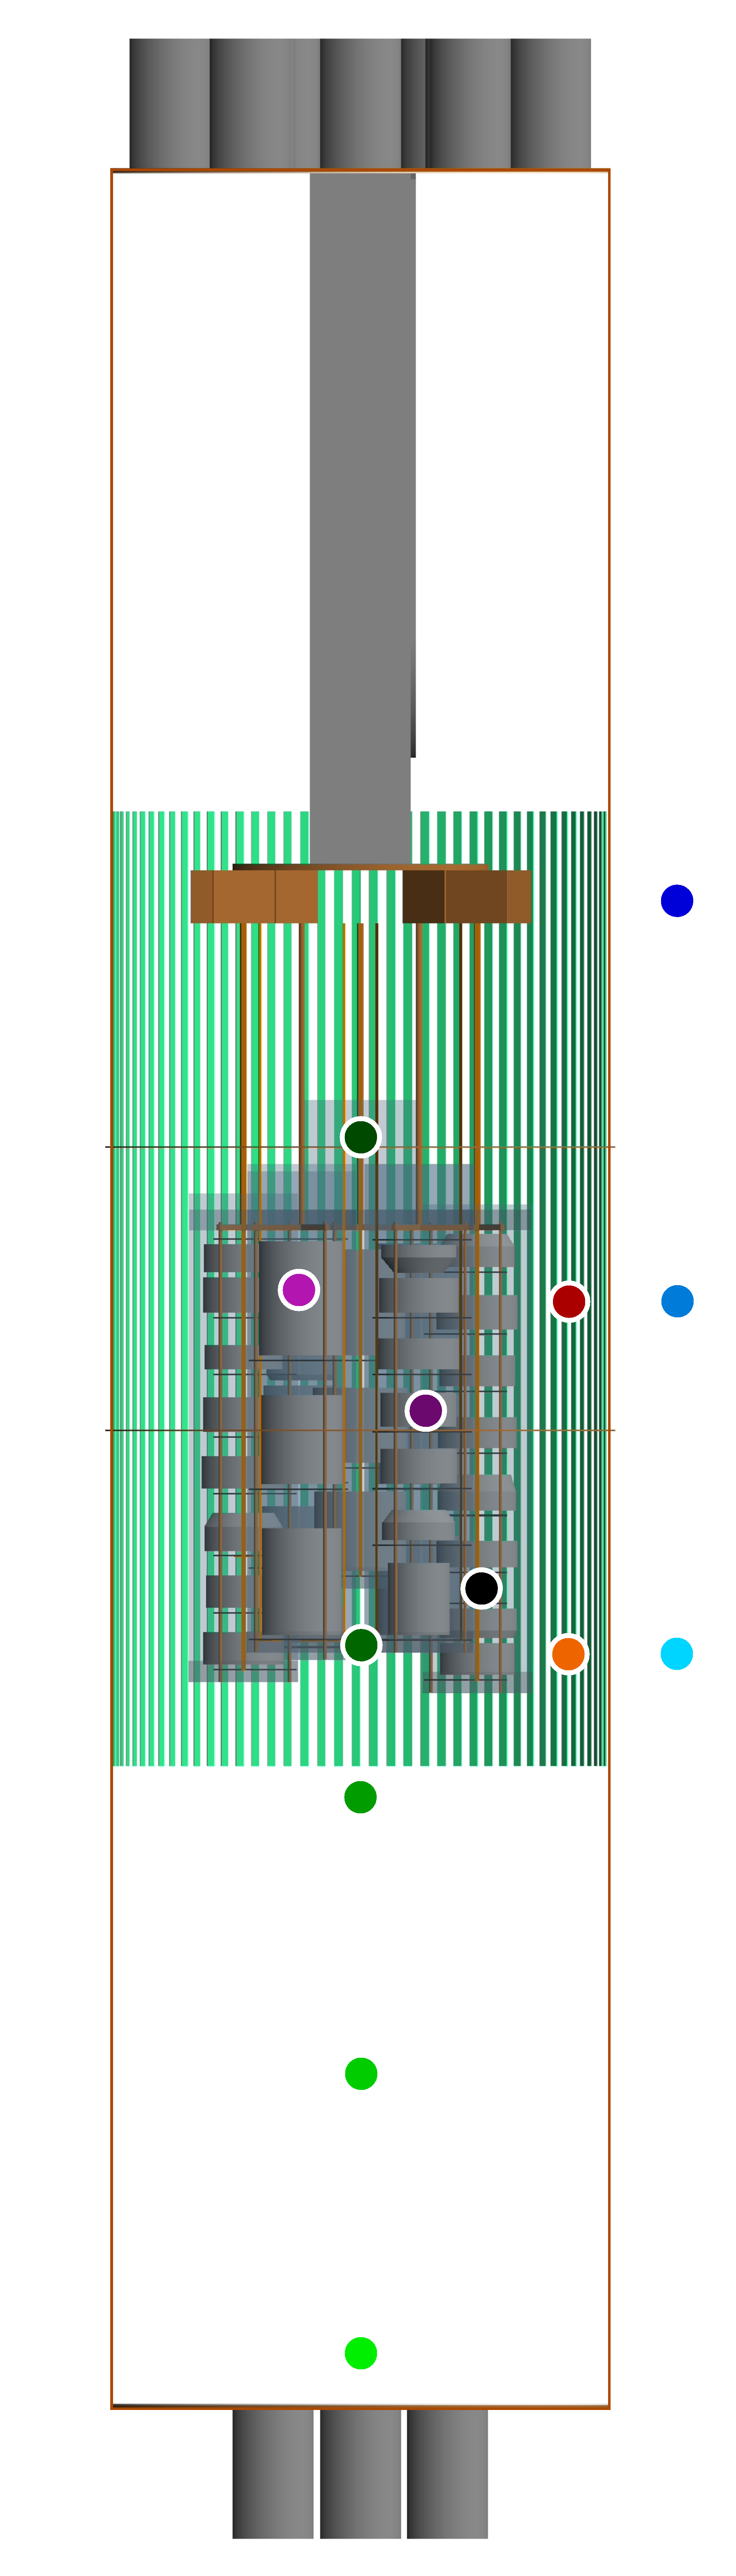
\includegraphics[height=0.8\textwidth, angle=90]{plots/bkg/lar/ph2/larmodel/lar-points-position.pdf}
  \includegraphics{plots/bkg/lar/ph2/larmodel/larmap-dist.pdf}
  \caption{%
    Study of the impact of Monte Carlo parameters on LAr light detection probabilities in
    various spatial points. Each curve shows the dependence of the probability upon
    germanium reflectivity, fiber shroud coverage and LAr absorption length in the points
    shown in the rightmost scheme of the \gerda\ setup, using the same color code. The
    germanium reflectivity is scaled by a global factor, such that the unit value
    corresponds to the value implemented in \mage. \fillme{check this plot}
  }\label{fig:bkg:lar:ph2:larmap:dist}
\end{figure}

\subsection{Tuning the LAr veto Monte Carlo model}%
\label{sec:bkg:lar:ph2:pcalib}

As already mentioned several times, the knowledge about several Monte Carlo optical
specifications is very limited. In particular, PMT and SiPM channel efficiencies are not
known and are essential to build a predictive LAr veto model. Efficiencies extracted from
physics data cannot be used directly, as the Monte Carlo efficiencies are in reality
complex objects that account for other effects. As instance, SiPM efficiencies can include
systematic effects from details of the geometry implementation of the fiber modules in
\mage. To overcome these issues, a statistical analysis has been developed to tune the
Monte Carlo parameters with physics data. A sample which is independent from the
regular \gerda\ physics data has been identified in the special calibration runs with
low-activity sources and the LAr veto instrumentation turned on. A short overview of this
analysis will be given in this section, the reader is referred to~\cite{Wiesinger2021} for
an extensive presentation of this broad subject.

\blocktitle{pcalib \\ runs}
The main characteristics of these data sets are documented in
\cref{tab:bkg:lar:ph2:pcalib-desc}: the first special run carries identification number
equal to 68 and has been performed with a \Th\ source in July 2016, while the second one
is run 76 and has been carried through in February 2017 with a \Ra\ source. Data has been
acquired with the sources \m{S2} and \m{S3} at three vertical positions at the top, middle
and bottom of the array. The lower source activity ($\mathcal{O}$(kBq)) makes it possible
to collect data with also the LAr veto instrumentation and provide a distinct setting for
an accurate data-to-Monte-Carlo comparison. Since the subject of this study are the
vetoing capabilities of the LAr system, the germanium main trigger has been maintained
during the data taking. Test pulses are also available and are used to estimate the
fraction of `random coincidences'. In these particular `false-positive' LAr-vetoed events
the physical process generating the scintillation light detected by PMTs and SiPMs is
distinct from the one triggering the germanium detectors at the same time. This can
happen, for example, if a calibration source decay product deposits some energy in the
germanium while a cosmic ray is ionizing the argon. Similarly these random coincidences
can be produced by two nuclear decays happening at the same time. A good estimate of the
random coincidences fraction in this special calibration data is crucial when comparing to
simulations, which miss this background-like component. Unfortunately, as documented in
\cref{tab:bkg:lar:ph2:pcalib-desc}, test pulse data is partly missing in run 68.

\begin{table}
  \centering
  \caption{%
    Summary of the special calibration data with active LAr veto instrumentation from runs
    68 (July 2016, \Th\ source) and 76 (February 2017, \Ra\ source). The random
    coincidences are estimated combining data from test pulses and SiPM
    traces~\cite{Wiesinger2021}.
  }\label{tab:bkg:lar:ph2:pcalib-desc}
  \begin{tabular}{lcccc}
    \toprule
    isotope      & source port & position (mm) & run time (h) & random coincidences (\%) \\
    \midrule
    \mr{6}{\Th}  &             & 8168          & 10.2         & --                       \\
                 & \m{S2}      & 8396          & 3.2          & --                       \\
                 &             & 8570          & 12.5         & --                       \\
                 \cmidrule{2-5}
                 &             & 8220          & 6.4          & $7.5 \pm 0.6$            \\
                 & \m{S3}      & 8405          & 4.3          & $7.2 \pm 1.0$            \\
                 &             & 8570          & 3.6          & $10.2 \pm 1.4$           \\
    \midrule
    \mr{6}{\Ra}  &             & 8139          & 8.9          & $12.2 \pm 0.3$           \\
                 & \m{S2}      & 8405          & 4.3          & $11.2 \pm 0.4$           \\
                 &             & 8570          & 6.9          & $12.9 \pm 0.3$           \\
                 \cmidrule{2-5}
                 &             & 8128          & 8.0          & $10.8 \pm 0.3$           \\
                 & \m{S3}      & 8292          & 3.6          & $8.9 \pm 0.4$            \\
                 &             & 8570          & 8.5          & $10.7 \pm 0.3$           \\
    \bottomrule
  \end{tabular}
\end{table}

\blocktitle{data \\ selection}
The analysis data set is constructed by applying an event cut based on the total energy
released in the germanium detectors. The selected energy regions are shown in
\cref{fig:bkg:lar:ph2:pcalib-data}: the \Tl\ FEP events ($2615 \pm 10$~keV) in run 68 and
the Compton-dominated energy region from 2204~keV \Bih\ line in run 76 are considered. The
obtained statistics is of about $2 \cdot 10^4$ events or more per source position.
\newpar
The data from the LAr instrumentation which is relevant to the comparison with the Monte
Carlo simulation consists in a set of veto flags (one for each of the 25 LAr veto
channels, i.e.~9 top PMTs, 7 bottom PMTs and 9 SiPM modules) for each germanium trigger.
The probability that a LAr veto channel is triggered in data can be written as the
convolution between a `signal' probability (the same event is responsible for both the
germanium and LAr veto triggers) and a `background' probability (the false-positive rate
from random coincidences). This convolution is simply the logic OR between the two
probabilities. The amount of random coincidences is estimated by combining data from test
pulses and SiPM traces, as documented in great detail in~\cite{Wiesinger2021}.

\begin{figure}
  \centering
  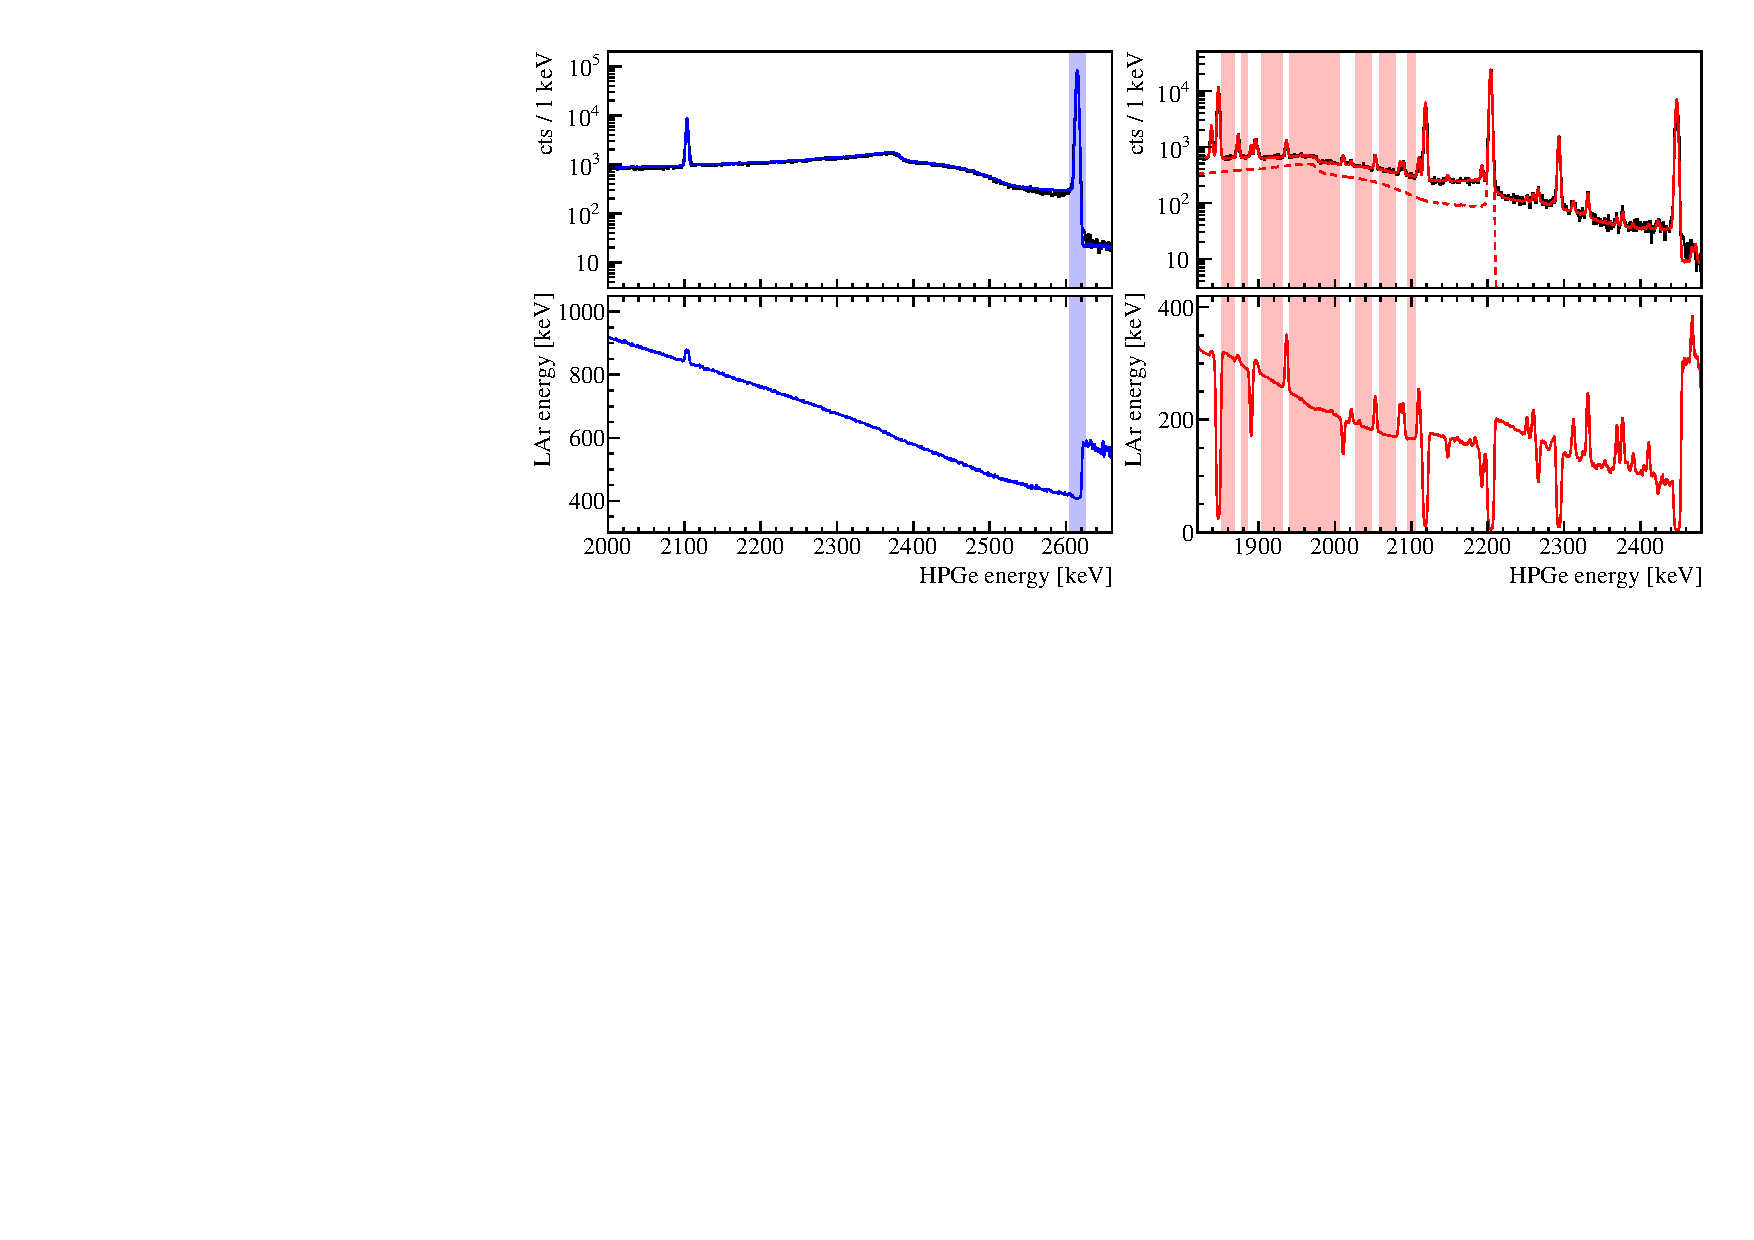
\includegraphics[width=0.9\textwidth]{plots/bkg/lar/ph2/larmodel/pca-analysis-window.pdf}
  \caption{%
    The energy spectra of the \phasetwo\ special calibration runs. Left: run 68 (\Th),
    Monte Carlo simulation in blue and data in black. The top panel shows the energy
    distribution of the events while the top panel shows the amount of average amount of
    energy released by an event with respect to its energy. Right: run 76 (\Ra). Colored
    bands highlight the regions selected for the data analysis.
  }\label{fig:bkg:lar:ph2:pcalib-data}
\end{figure}

\blocktitle{simulations}
The calibration sources are fully implemented in \mage, with user commands to set their
vertical position, the radioactive source and therefore replicate the run 68 and 76
experimental settings (\cref{tab:bkg:lar:ph2:pcalib-desc}). Optical
processes are enabled in these special simulation runs, but since they require high
computational time photons are fully tracked only if an energy deposition is recorded in
germanium as well. The optical properties of the setup are fixed to their best values
documented in \cref{sec:bkg:lar:ph2:mage}. The two most important Monte Carlo settings
for the calibration source physics are the LAr attenuation length and the fiber shroud
coverage. As demonstrated in \cref{sec:bkg:lar:ph2:heatmap} and in
\cref{fig:bkg:lar:ph2:larmap:dist} in particular, these are the two parameters that affect
the most the LAr light detection probability in the red and orange points --- where the
calibration sources are typically deployed. The germanium reflectivity, instead, is
crucial when probing the region of the array. Changes in the LAr light yield or the TPB
quantum efficiencies produce nearly linear distortions of the probability map and can be
absorbed in the PMT and SiPM channel efficiencies.

\blocktitle{statistical \\ analysis}
The probability to detect $n$ LAr scintillation photons with the LAr veto instrumentation
includes a signal component (the light is physically correlated to the germanium signal)
and a background component from random coincidences:
\[
  \lambda[n] = \lambda_s[n] * \lambda_b[n] = \lambda_s \vee \lambda_b \;.
\]
A way to introduce an effective detection efficiency $\epsilon$ for a LAr veto channel is
by the following `binomial repopulation':
\[
  \lambda_s[m](\epsilon) = \sum_{n \geq m} \lambda_s[n] \binom{n}{m} \epsilon^m
    {(1-\epsilon)}^{n-m} \;,
\]
which is the probability, reduced by the efficiency $\epsilon \in [0,1]$, to observe $m <
n$ photons. Since the quantity of interest for this analysis is the LAr veto flag (i.e.~an
event is seen by the instrumentation or not), the probability to detect $m > 0$ photons
can be expressed as
\[
  \lambda_s(\epsilon) = 1 - \lambda[0](\epsilon)
                      = 1 - \sum_n \lambda_s[n] {(1-\epsilon)}^n
                      = 1 - \frac{1}{N_\text{tot}} \sum_n N_n {(1-\epsilon)}^n \;,
\]
where the last equality holds for the Monte Carlo simulations, in which $\lambda_s[n]$ is
just the ratio between the number of events in which $n$ photons were detected and the
total number of events: $\lambda_s[n] = N_n / N_\text{tot}$.
\newpar
A likelihood function is then constructed to match the Monte Carlo simulation output to the
special calibration data. Since each single event includes data from 25 LAr veto channels,
also the particular `detection pattern' must be taken into account. Given three channels
$A$, $B$ and $C$, for example, the pattern $\{A,C\}$ represents the occurence of a signal
in channel $A$, $C$ but not in $B$. The pattern in the example has probability $p_A
\cdot (1-p_B) \cdot p_C$, i.e.~it always probes all the channel detection probabilities
$p_i$. The full likelihood reads
\begin{equation}\label{eq:bkg:lar:ph2:pca-likelihood}
  \mathcal{L}(\vec{\epsilon}, \ldots) =
    \prod_P \operatorname{B}_{N_\text{tot}}^N \big(
      \sum_G ( \lambda_s(\vec{\epsilon}) + \sigma \cdot \Delta\lambda_s(\vec{\epsilon})) \cdot
      \lambda_b \big)
    \cdot \prod_G \operatorname{B}_{M_\text{tot}}^M (\lambda_b) \cdot
    \operatorname{G}(\sigma) \;,
\end{equation}
where the first product runs over all possible $\dim{P} = 2^{N_\text{ch}}$ patterns
($N_\text{ch}$ is the number of considered channels), the summation and the last product
run over all the pattern generator pairs $G = \{\{A,B\},\{B,C\},\ldots\}$. In the first
binomial term $\operatorname{B}^N_{N_\text{tot}}(\lambda)$, $N$ is the number of events in
which light was seen over the total $N_\text{tot}$ for a certain pattern. The same
nomenclature applies for the second binomial term
$\operatorname{B}^M_{M_\text{tot}}(\lambda)$, but now for the random coincidence data set.
The probability in the first binomial term is the product between the signal probability
for a given pattern (which is calculated by summing over all possible pattern generators)
and the background random coincidence probability $\lambda_b$. The signal probability
contains an additional contribution $\sigma \Delta\lambda_s(\vec{\epsilon})$ which
accounts for the effect of low statistics in the Monte Carlo data sample. The term is
regulated by the nuisance parameter $\sigma$, which is constrained by the pull term
$\operatorname{\sigma}$, a Gaussian distribution with null mean and variance $\sigma$. The
number of degrees of freedom of this likelihood is $2^{N_\text{ch}}-N$.
\newpar
The likelihood function is then maximized to obtain the best fit values for the parameters
of interest, the LAr veto channel efficiencies $\vec{\epsilon}$. The same likelihood
function can also be used to make some inference on other Monte Carlo optical unknowns,
e.g.~the LAr attenuation length or the fiber shroud coverage. This idea is presented and
discussed in~\cite{Wiesinger2021}, but its application is out of the scope of this work,
which requires only a rough tuning of the LAr probability map. Indeed, a broad range of
systematic map distortions which might be due to uncertain optical specifications is
tested in the framework of the \nnbb\ distribution analysis, which will be presented in
\cref{chap:2nbb-ana}.

\blocktitle{results}
Since the tuned LAr probability map will be only used to provide the LAr veto flag for the
background model simulations, which are further processed to create the pdfs for the
\bege\ summed energy spectrum, an additional simplification can be introduced in the
analysis. In principle, the array of channel efficiencies $\vec{\epsilon}$ in
\cref{eq:bkg:lar:ph2:pca-likelihood} has dimension 25, but the symmetries of the
experimental setup can be exploited to reduce the number of parameters. A cylindrical
symmetry is \emph{de facto} present in the arrangement of PMTs and SiPM modules, as shown
in the technical drawings in \cref{fig:setup:magevolumes}. This spatial symmetry is evidently
broken in the LAr veto channel efficiencies domain, since the measured signal rates are
already different one from the other, but the effect of this asymmetry has to be evaluated
on the analysis data set, i.e.~the \bege\ summed energy spectrum. Since the \bege\
detector arrangement in the array does not significantly deviate from a cylindrical
distribution, it is not expected to depend too much on differences between efficiencies of
light detectors at the same vertical height. Therefore, only three effective efficiencies
are used in \cref{eq:bkg:lar:ph2:pca-likelihood} ($N_\text{ch}=3$): one for all top PMTs,
one for all SiPM modules and one for all bottom PMTs.
\newpar
In this simplified setting, the maximization of $\mathcal{L}(\vec{\epsilon})$ yields:
\begin{equation}\label{eq:bkg:lar:ph2:chan-eff}
  \epsilon_\text{PMTt} = 0.140 \pm 0.003 \;, \quad
  \epsilon_\text{SiPM} = 0.326 \pm 0.007 \;, \quad
  \epsilon_\text{PMTb} = 0.346 \pm 0.007 \;.
\end{equation}
And the magnitude of systematic uncertainty needed to obtain a reasonable goodness of fit
($-2\Delta\log\mathcal{L}=10$) at the best fit point is around 30\%, which already shows
how this analysis suffers from the many unknown optical specifications in the Monte Carlo.
The impact of this problem on the \nnbb\ distribution analysis is addressed in
\cref{sec:2nbb-ana:systematics} through a dedicated study of the connected systematic
uncertainty.

The background model pdfs after LAr veto cut obtained by applying the probability map to
the Monte Carlo simulations (the same used to produce the pdfs before analysis cuts shown
in \cref{fig:bkg:raw:ph2:pdfs:gmodel}) are displayed in
\cref{fig:bkg:lar:ph2:pdfs:gmodel}. Another notable difference with the pdfs constructed
for the analysis presented in \cref{chap:bkg:raw:ph2} is that the linear transition layer
model obtained from characterization data for \bege\ detectors \cite{Lehnert2016} is now
taken into account. More information about the germanium detector transition layer models
is found in \cref{apdx:gedetav}. \fillme{any other comment?}

\begin{figure}
  \centering
   \subfloat[\label{fig:bkg:lar:ph2:pdfs:gmodel:Th}%
     \Bil\ and \Tl\ (\Thh\ chain) contaminations far from (fiber shroud) and close to
     (mini-shrouds) the detectors.
   ]{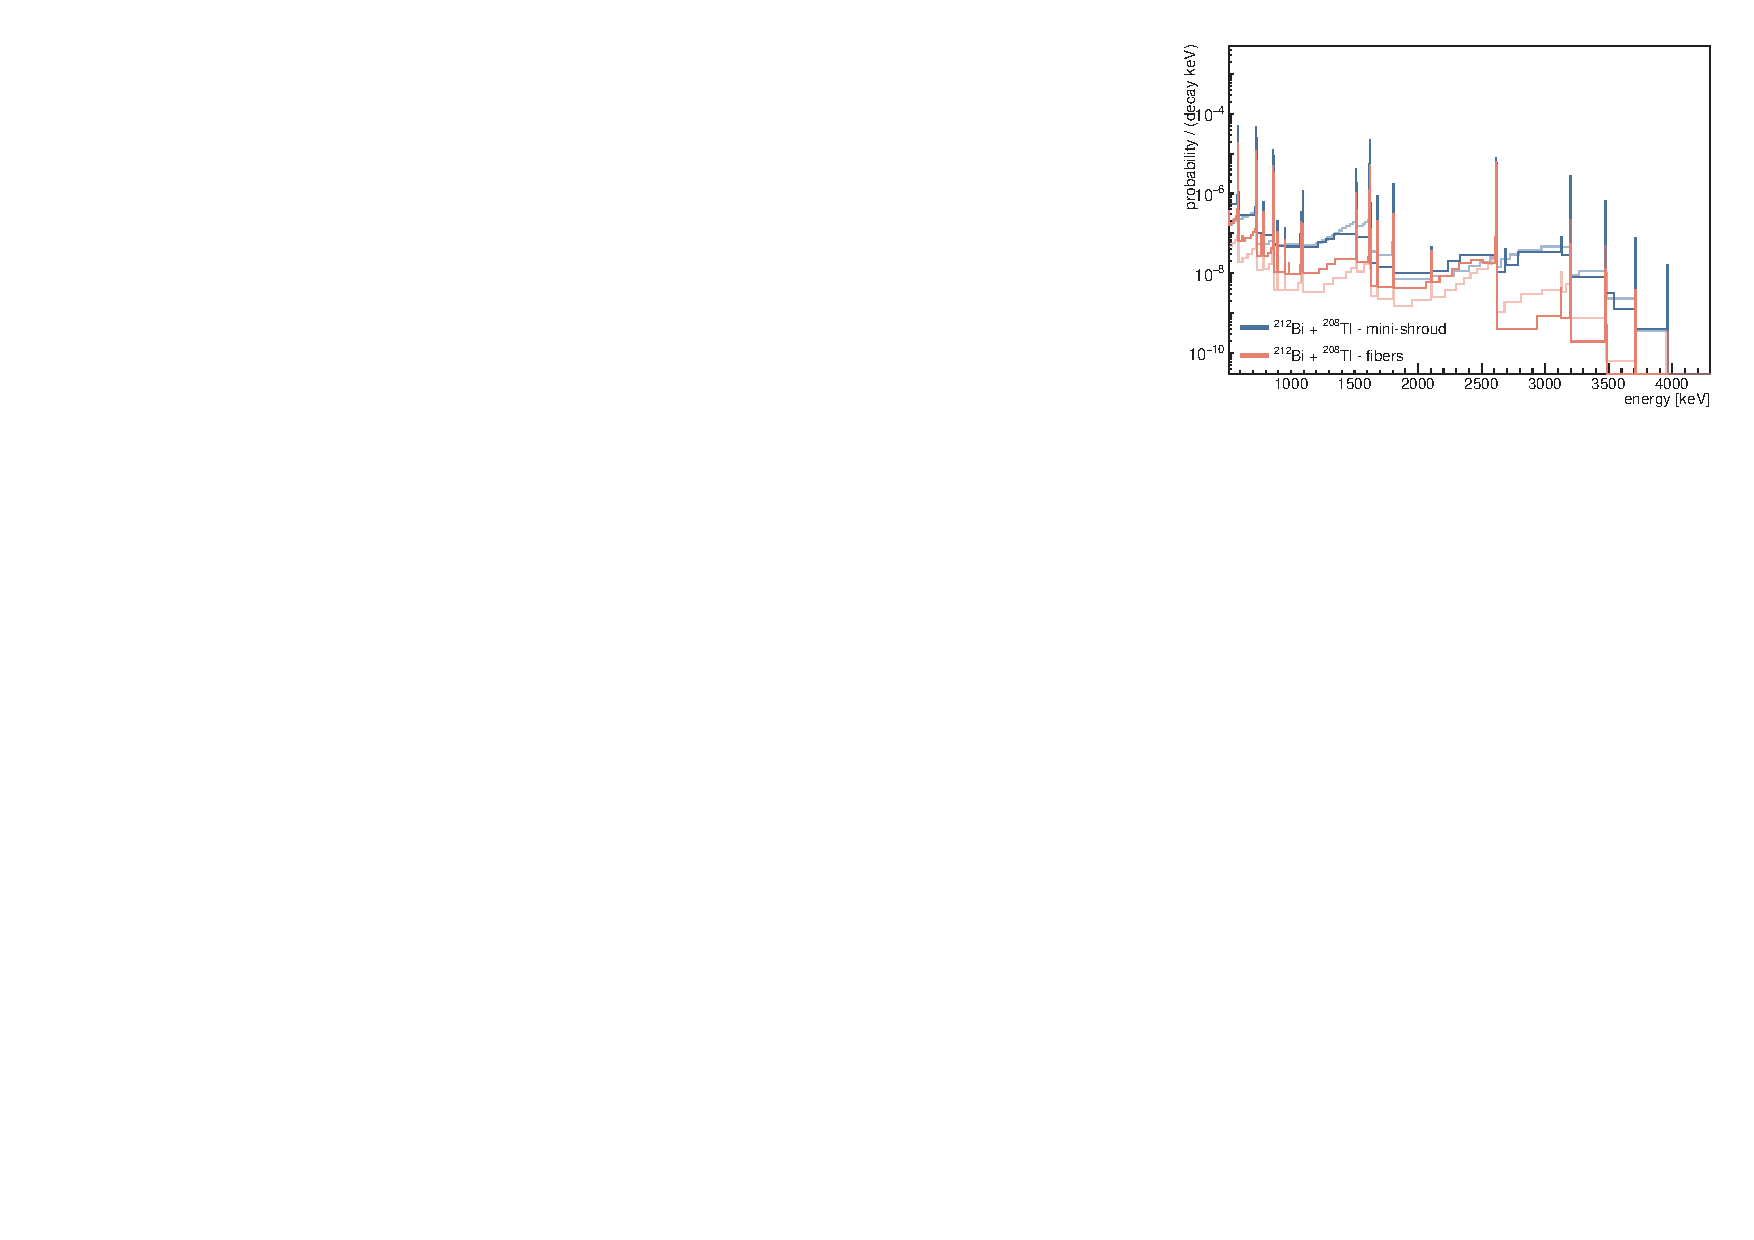
\includegraphics[width=0.48\textwidth]{plots/bkg/lar/ph2/pdfs/gmodel-pdfs-Th.pdf}}
   \hfill
   \subfloat[\label{fig:bkg:lar:ph2:pdfs:gmodel:U}%
     \Bih\ and \Pbh\ (\Uh\ chain) contaminations far from (fiber shroud) and close to
     (mini-shrouds) the detectors. \fillme{simulate also far?}
     ]{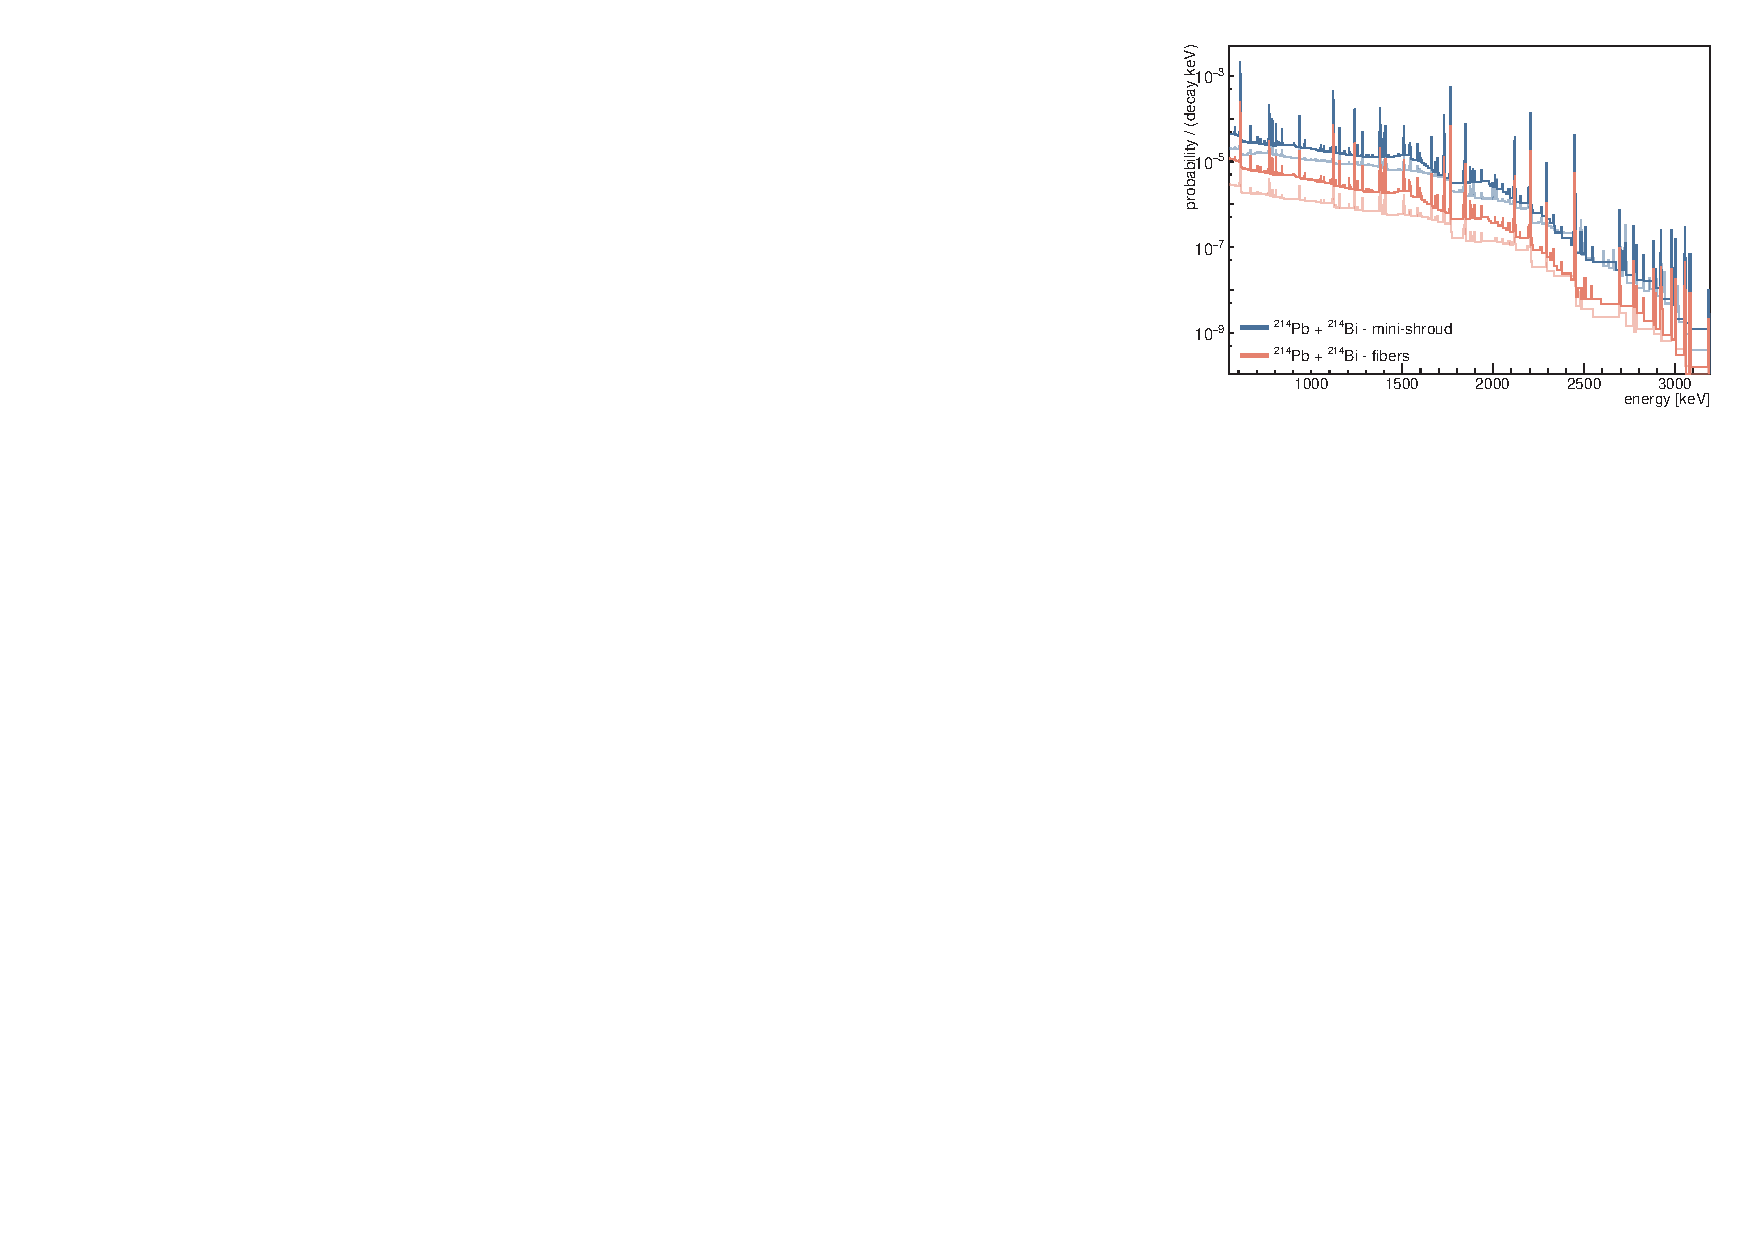
\includegraphics[width=0.48\textwidth]{plots/bkg/lar/ph2/pdfs/gmodel-pdfs-U.pdf}}

  \subfloat[\label{fig:bkg:lar:ph2:pdfs:gmodel:K40}%
    \kvn\ contamination close to the detectors (mini-shrouds), at a higher radial distance
    (fiber shroud) and higher vertical distance (copper shrouds).
  ]{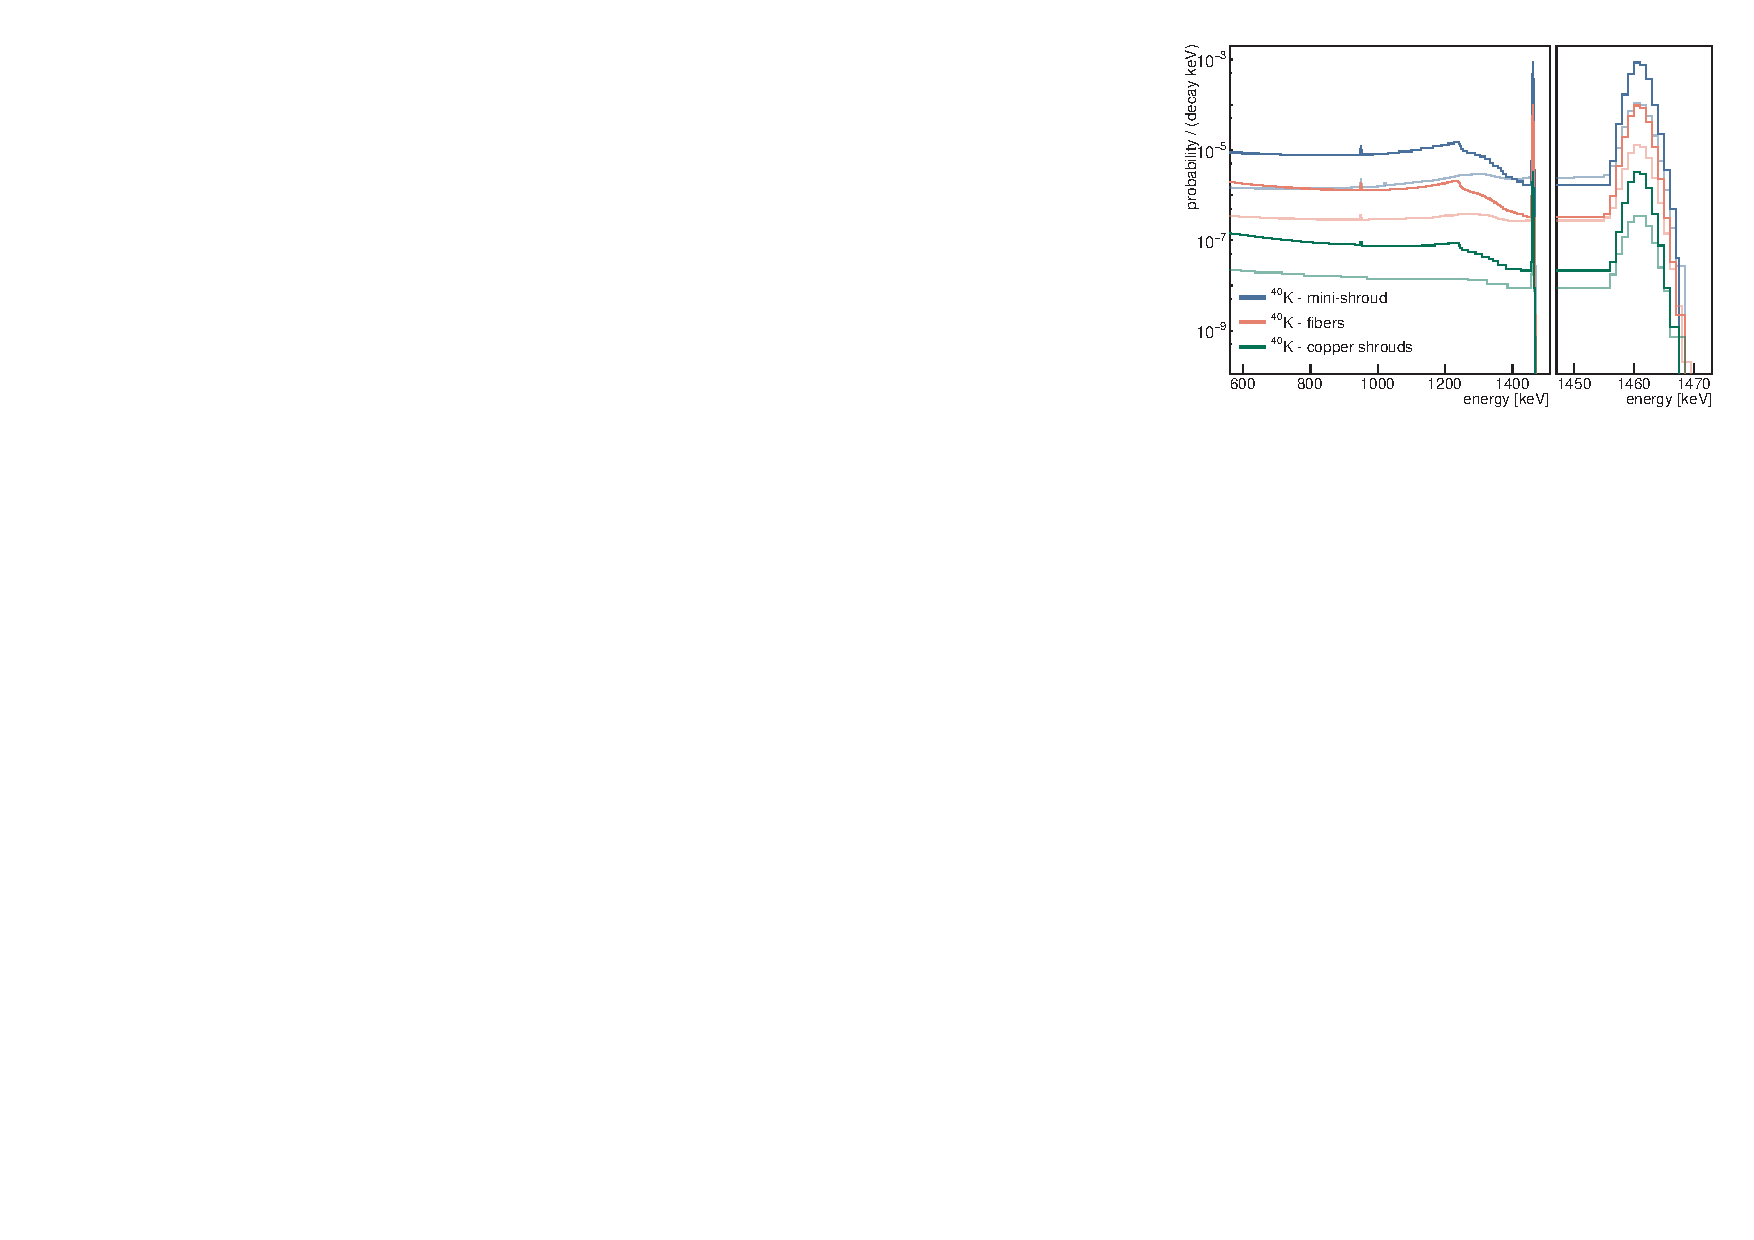
\includegraphics[width=0.48\textwidth]{plots/bkg/lar/ph2/pdfs/gmodel-pdfs-K40.pdf}}
  \hfill
  \subfloat[\label{fig:bkg:lar:ph2:pdfs:gmodel:K42}%
    \kvz\ contamination in different locations inside the LAr.
  ]{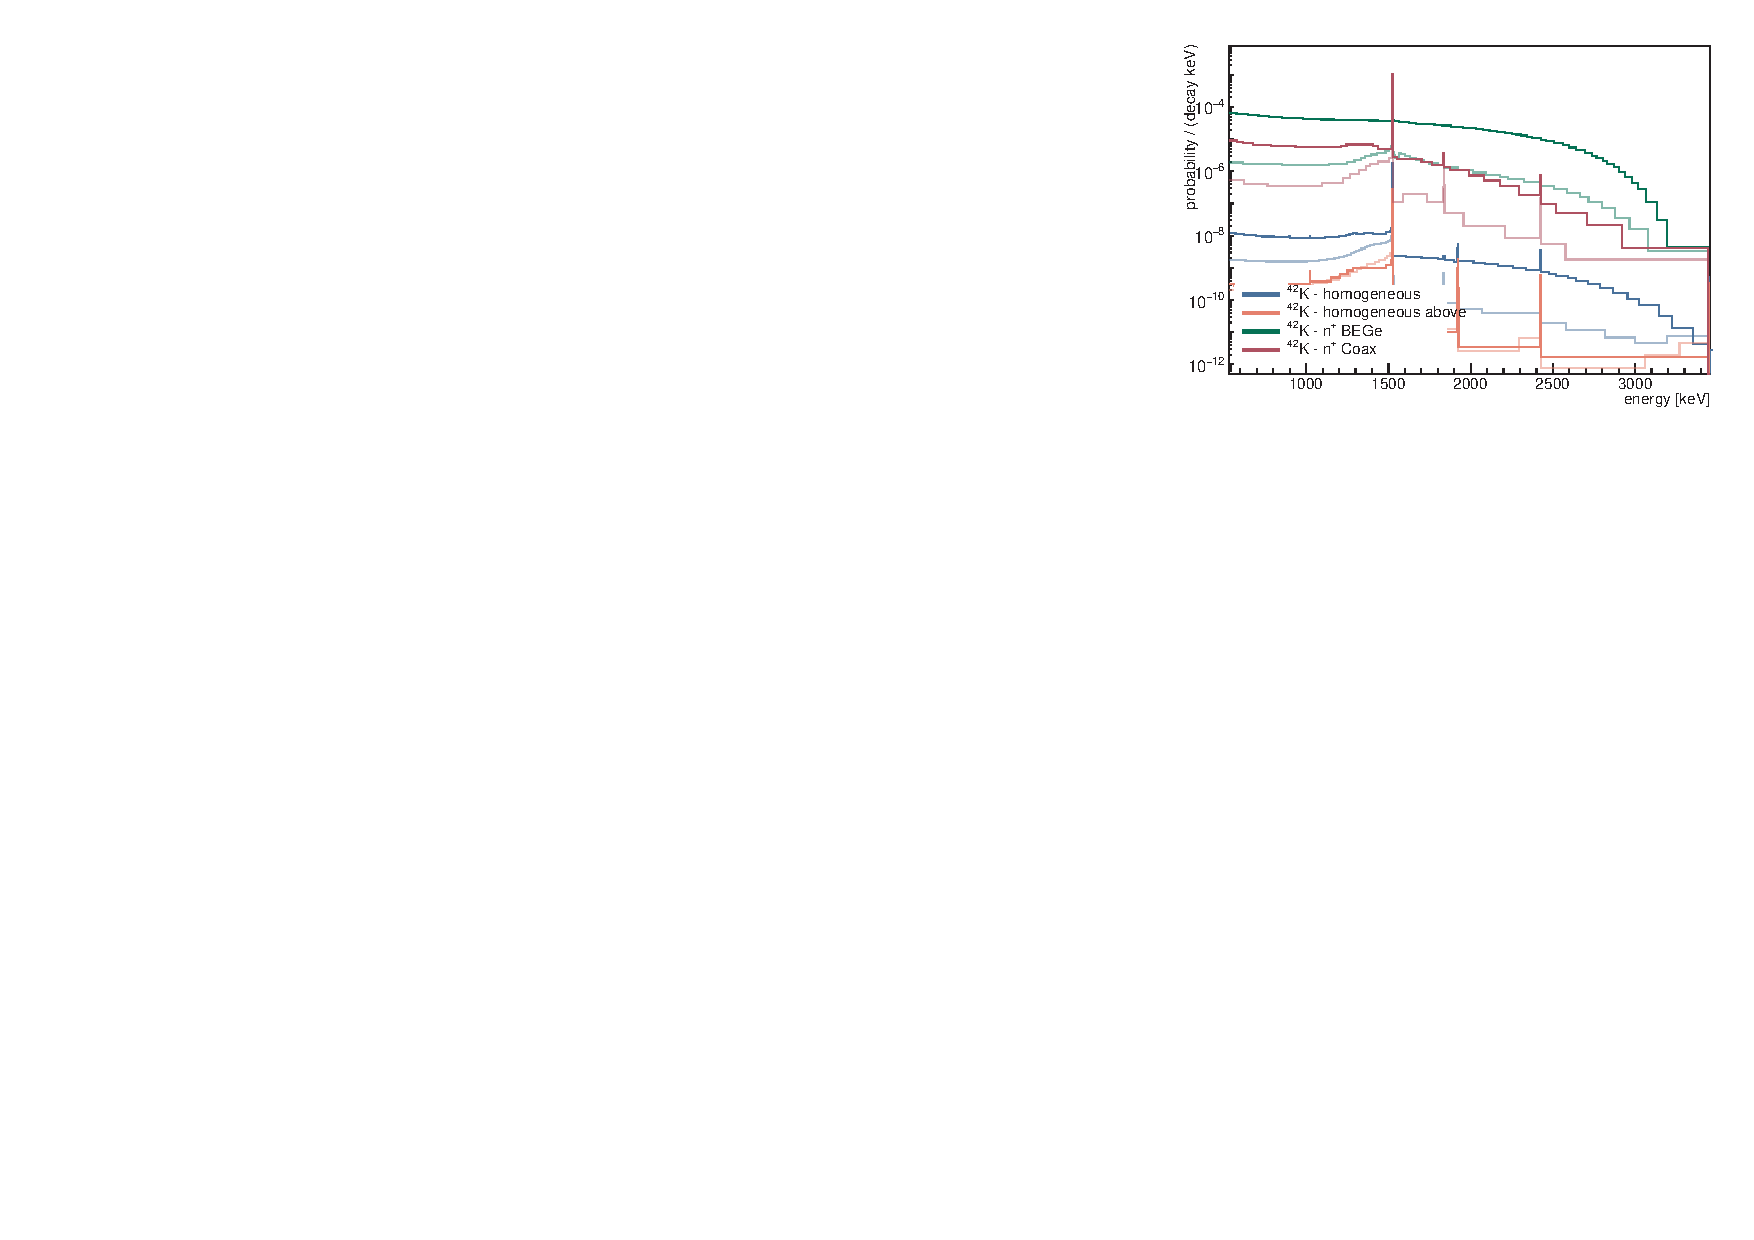
\includegraphics[width=0.48\textwidth]{plots/bkg/lar/ph2/pdfs/gmodel-pdfs-K42.pdf}} \\

   \subfloat[\label{fig:bkg:lar:ph2:pdfs:gmodel:other}%
   \Ac\ contamination in the close vicinity of the detectors (mini-shrouds).
   ]{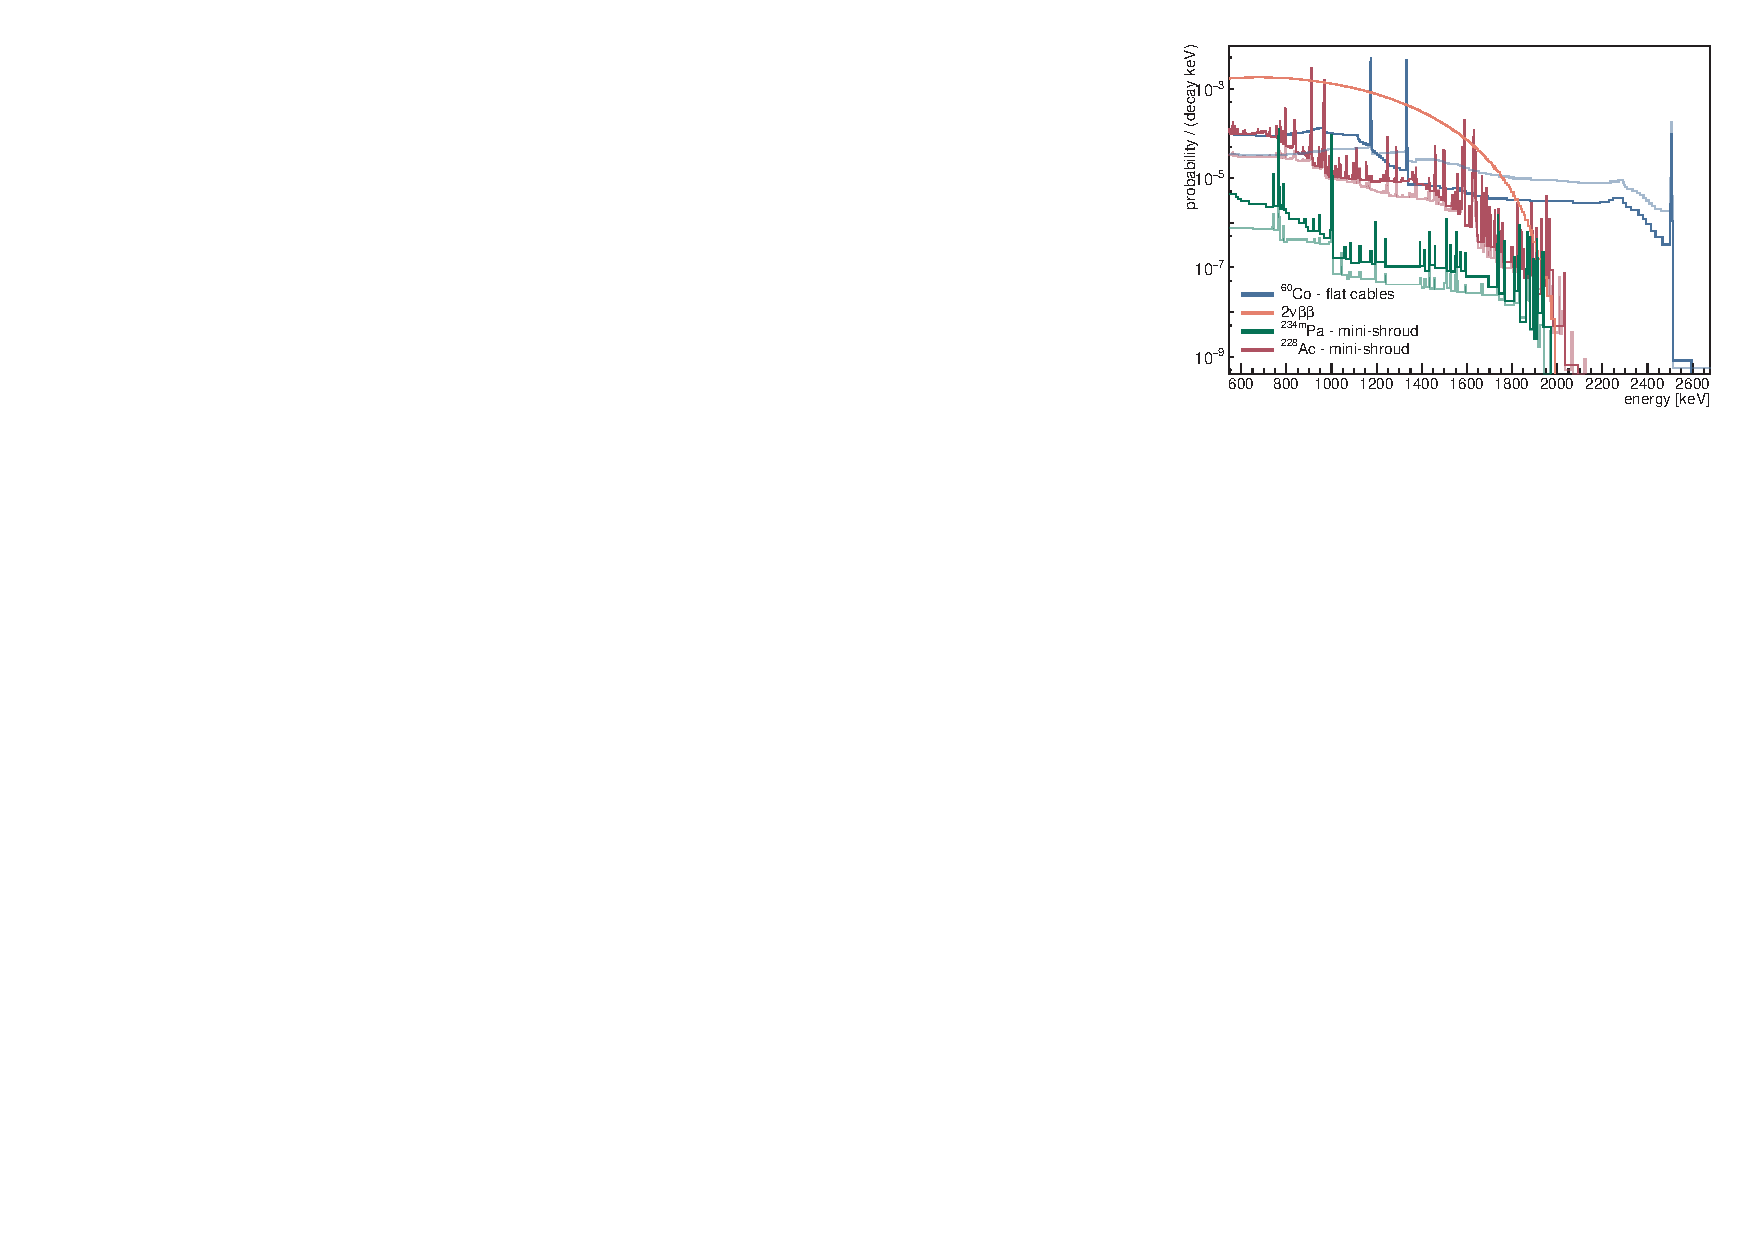
\includegraphics[width=0.48\textwidth]{plots/bkg/lar/ph2/pdfs/gmodel-pdfs-misc.pdf}}
   \hfill
   \subfloat[\label{fig:bkg:lar:ph2:pdfs:gmodel:other2}%
     \Co\ contamination in the signal and high-voltage cables and detector intrinsic
     \gesix\ \nnbb\ decay.
   ]{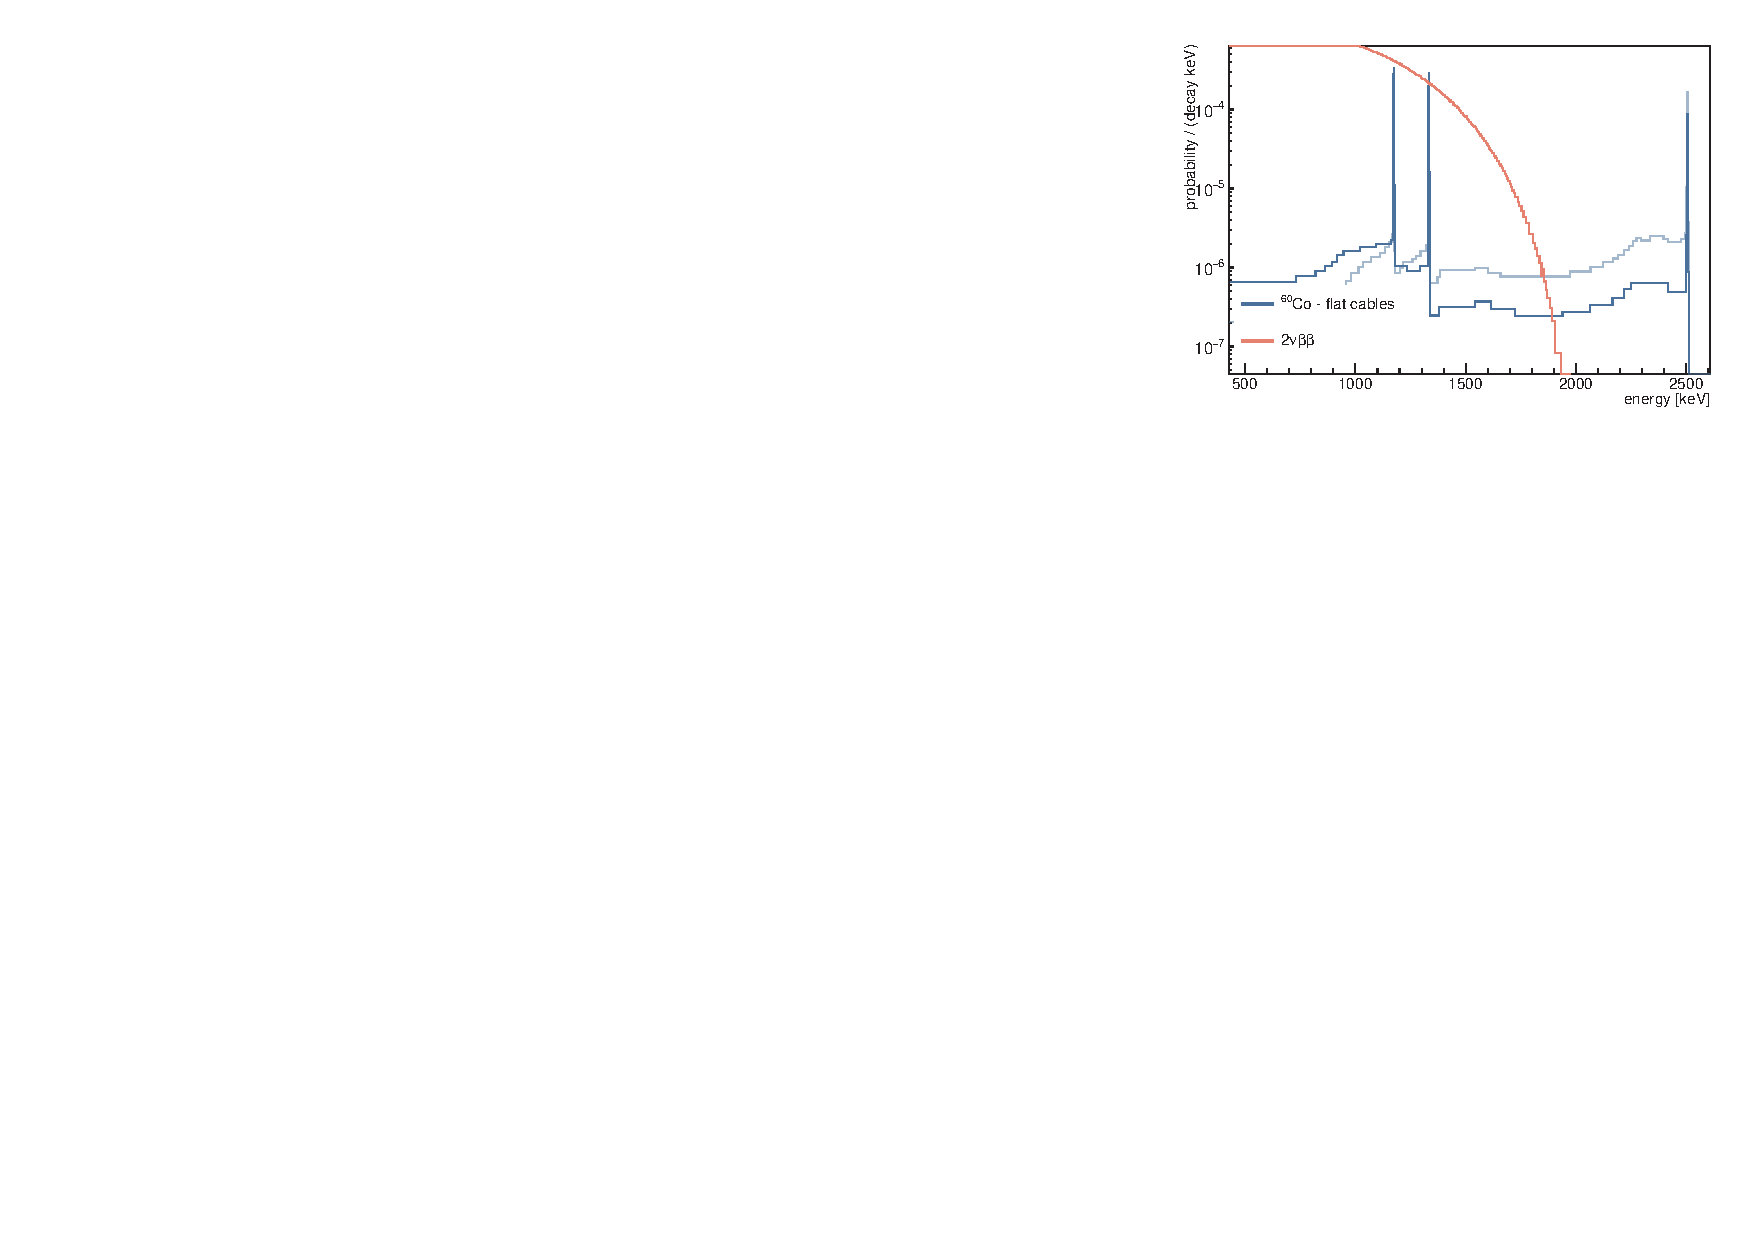
\includegraphics[width=0.48\textwidth]{plots/bkg/lar/ph2/pdfs/gmodel-pdfs-misc2.pdf}}

  \caption{%
    The pdfs for the \enrGeII\ ($\enrBEGeII + \enrCoaxII$) (in fully opaque colors) and
    the \enrGeII\ (in shaded colors) data sets after the LAr veto cut in the full energy
    domain and relative to different background sources. Bayesian blocks are used to
    visualize histograms (see \cref{apdx:bayesblocks} for details. All pdfs are normalized
    to the number of simulated events. These pdfs should be compared with those before the
    LAr veto cut in \cref{fig:bkg:raw:ph2:pdfs:gmodel}.
  }\label{fig:bkg:lar:ph2:pdfs:gmodel}
\end{figure}

\section{Full-range analysis}%
\label{sec:bkg:lar:ph2:gmodel}

A full-range background analysis of the energy spectra after the LAr veto cut in the same
spirit of the one reported in \cref{sec:bkg:raw:ph2:gmodel} has been carried on. The
\a-event analysis has not been repeated, as they survive almost completely the LAr veto
cut.  The pdfs extracted from the \a\ model presented in \cref{sec:bkg:raw:ph2:amodel} can
be therefore used in the full-range analysis as they are. The potassium tracking analysis
has not been repeated too.

\blocktitle{statistical \\ methods}
The full-energy spectrum has been analysed in its entire range from 565~keV to 5260~keV
and no data sub-sets have been excluded. To speed-up the analysis and exploit all the
information brought by data at the same time, an heuristic variable binning has been
adopted. Dedicated bins have been used for the strongest \g\ lines: the two \kvn\ and
\kvz\ lines, the \Bih\ and \Tl\ lines. In the rest of the energy spectrum the bin size has
been chosen according to the event rate (e.g.~10~keV for \enrBEGeII\ and \enrCoaxII\ above
the \Arl\ Q-value and below the potassium lines, 40~keV for \enrGeII). Since above the
\Tl\ FEP the \Mone\ event spectrum is dominated by \a\ events which are almost completely
surviving the LAr veto cut, only two bins $[2610, 4500]$~keV and $[4500, 5260]$~keV have
been set. As a cross-check, fit results have been tested to be stable when using this
data partitioning scheme or a fixed 5~keV binning.
\newpar
The statistical analysis to determine the background decomposition consists in the usual
Poisson likelihood maximization in a Bayesian setting presented in
\cref{sec:bkg:raw:ph2:stat}. The C++ BAT-based~\cite{Caldwell2008} software routine is
publicly available on GitHub\textsuperscript{\ref{footnote:gerda-fitter}}. Since the
global event suppression factor built in the pdfs after the LAr veto cut (i.e.~the pdf
normalization) cannot be fully trusted\footnote{%
  \fillme{A nice way to explain this? Ask Christoph}
}, no priors from screening measurement data have been set. A uniform prior is assigned to
all fit parameters (including the \nnbb\ fit parameter, which is proportional to
$1/\thalftwoM$).

\blocktitle{results}
Since the background level (excluding the \a\ events) is about an order of magnitude less
than before the LAr veto cut, a basic sample of background pdfs has been tested in the fit
model. Given the reduce size of the background sample, in fact, no sensitivity to
second-order shape distortions between pdfs of the same radioactive decay in different
locations (e.g.~\Ac\ in holders, cables, etc.) is expected. The following set of pdf
components has been therefore selected: \nnbb\ in germanium, \kvn\ close (mini-shrouds)
and far (fiber shroud) from the detectors, \kvz\ close (on the \bege\ and \scoax\ \nplus\
contact, in the LAr inside the mini-shrouds) and far (in the LAr outside the
mini-shrouds, in the LAr above the array), \Bil\ and \Tl\ on cables, \Pbh\ and \Bih\ on
cables, \Co\ on cables, \Ac\ on detector holders and the \a\ model pdfs for \bege\ and
\scoax\ detectors from \cref{sec:bkg:raw:ph2:amodel}.
\newpar
Not all the marginalized posterior distributions of fit parameters report non-zero
estimates of background counts in the spectra. Notably, posteriors for \kvz\ above the
array and on the \bege\ \nplus\ contact are peaked at zero and are thus removed from the
fit. The exclusion of \kvz\ on the \bege\ \nplus\ contact, which has not been reported in
the fit before analysis cuts (\cref{chap:bkg:raw:ph2}), is attributed to the novel
transition layer model, which significantly affects the pdf shape above the full-energy
peak. The \b\ spectrum component above 1525~keV, indeed, is now higher and shows less
compatibility with experimental data. The \Co\ component is also compatible with zero,
possibly because of the high LAr veto efficiency on a background contamination which was
already low before the cut (see \cref{tab:bkg:raw:ph2:gmodel:results}). Nevertheless,
the component is not removed from the fit because of its clear non-zero mode. Finally, a
strong anti-correlation is present between the two \kvn\ sources far and close to the
array. The former can be dropped from the model without affecting the fit results.
\newpar
The results of the analysis are shown in
\cref{fig:bkg:lar:ph2:results,fig:bkg:lar:ph2:results-fixbw,fig:bkg:lar:ph2:results-closeup}
and \cref{tab:bkg:lar:ph2:results}. Since the radioactivity of hardware parts is better
constrained within the background model before the analysis cuts
(\cref{chap:bkg:raw:ph2}), where the background level is higher, and additional
uncertainties affect the normalization of the pdfs after the LAr veto cut, only the
reconstructed number of counts in the fit range and the background index are given. The
background decomposition in \cref{fig:bkg:lar:ph2:results} is presented together with the
residuals plot and the 68\%, 95\% and 99\% central Poisson probability intervals of the
best fit model. Already from a visual inspection of the residuals, the goodness of fit is
not completely satisfactory through all the spectrum. In particular, discrepancies between
the best-fit model and the data are visible in \enrGeII\ right below the potassium peaks,
in \enrBEGeII\ around the potassium Compton shoulder region and in \enrCoaxII\ in the
$[1.8, 2]$~MeV region (\cref{fig:bkg:lar:ph2:results-closeup}).

\blocktitle{background \\ at \qbb}
The background model describes the individual contributions to the total background index
around \qbb\ after the LAr veto cut. The background index is defined as the number
of counts over exposure and energy in the energy window from 1930~keV to 2190~keV
excluding the region around \qbb\ ($\qbbM \pm 5$~keV) and the intervals $2104 \pm 5$~keV
and $2119 \pm 5$~keV, which correspond to known \g\ lines from \Tl\ and \Bih. The values
for each background contribution are given in \cref{tab:bkg:lar:ph2:results}. The
composition of the background around \qbb\ is also displayed as fractions of the total
background index in the following:
\begin{center}
  \includegraphics{plots/bkg/lar/ph2/results/gmodel/BI-bar.pdf}
\end{center}
The dominating background contribution in both data sets come from
\a\ decays, which are left practically untouched by the LAr veto cut. \kvz\ is the second
largest contribution, together with isotopes from the \Uh\ decay chain.
The estimated total
background indices extracted from the marginalized posterior distributions are
$\stat{6.22^{+0.47}_{-0.35}} \cdot 10^{-3}$~\ctsper\ for the \enrBEGeII\ data set and
$\stat{5.11^{+0.44}_{-0.32}} \cdot 10^{-3}$~\ctsper\ for the \enrCoaxII\ data set.

\begin{sidewaystable}
  \footnotesize
  \centering
  \caption{%
    Summary of the background decomposition after LAr veto cut. The number of
    reconstructed counts in the fit range and the BI at \qbb\ is listed for each component
    and each analysis data set. Marginalized modes, along with its smallest 68\% C.I., are
    reported as representatives of the marginalized posterior distributions.
  }\label{tab:bkg:lar:ph2:results}
  \newcolumntype{H}{>{\setbox0=\hbox\bgroup}c<{\egroup}@{}}
\newcolumntype{x}[1]{>{\centering\arraybackslash}p{#1}}
\newcommand{\mrr}[2]{\multirow{#1}[1]{*}{#2}}
\newcommand{\mrc}[2]{\multirowcell{#1}{#2}}

\begin{tabular}{%
  r
  l
  c
  S[% global mode
    table-format=4.2,
    table-number-alignment=right,
    table-text-alignment=right,
    table-parse-only
  ]
  r@{ }l% marginalized with 68% CI interval
  S[% screening measurements
    table-number-alignment=left,
    table-text-alignment=left,
    table-parse-only
  ]
  S[% BEGe
    table-format=5.0,
    table-number-alignment=center,
    table-text-alignment=center,
    table-auto-round=true
  ]@{ | }
  l
  S[% Coax
    table-format=4.0,
    table-number-alignment=center,
    table-text-alignment=right,
    table-auto-round
    ]@{ | }
  l
  S[% M2-All
    table-format=4.0,
    table-number-alignment=center,
    table-text-alignment=center,
    table-auto-round
  ]
}
  \toprule
  \mrr{3}{source}      & \mrr{3}{\m{[prior]} location}         & \mrr{3}{units}      & {\mrc{3}{global\\mode}} & \mc{2}{\mrc{3}{marg.~mode\\with 68\% CI}} & {\mrr{3}{screening}} & \mc{5}{model content in fit range | BI at \qbb}                                             \\
                       &                                       &                     &                         &       &                                   &                      & \mc{5}{units: cts | $10^{-3}$\ctsper}                                                       \\
  \cmidrule(lr){8-12}
                       &                                       &                     &                         &       &                                   &                      & \mc{2}{\enrBEGeII}                     & \mc{2}{\enrCoaxII}                     & \enrGeII\ \\
  \midrule
  \mr{2}{\nnbb}        & \m{[f]} \bege\ detectors              & \mr{3}{$10^{21}$yr} &                         &       &                                   & {--}                 &         & \mrc{2}{0}                   &         & \mrc{2}{0}                   &           \\
                       & \m{[f]} \scoax\ detectors             &                     &                         &       &                                   & {--}                 &         & \mrc{2}{0}                   &         & \mrc{2}{0}                   &           \\
                       & \m{[f]} \icoax\ detectors             &                     &                         &       &                                   & {--}                 &         & \mrc{2}{0}                   &         & \mrc{2}{0}                   &           \\
  \midrule
  \mr{3}{\Bil\ + \Tl}  & \m{[e]} flat cables                   & \mr{3}{$\upmu$Bq}   &                         &       &                                   & < 410                &         & \mrc{3}{3.52\\$[3.30,3.76]$} &         & \mrc{3}{2.21\\$[2.03,2.34]$} &           \\
                       & \m{[g]} copper shrouds$^{\dagger}$    &                     &                         &       &                                   & 194 \pm 19           &         &                              &         &                              &           \\
                       & \m{[g]} mini-shrouds                  &                     &                         &       &                                   & 18  \pm 5            &         &                              &         &                              &           \\
  \midrule
  \mr{6}{\Pbh\ + \Bih} & \m{[f]} \pplus\ (BEGe)                & \mr{6}{$\upmu$Bq}   &                         &       &                                   & {--}                 &         & \mrc{6}{2.63\\$[2.50,2.78]$} &         & \mrc{6}{3.16\\$[2.83,3.50]$} &           \\
                       & \m{[f]} \pplus\ (Coax)                &                     &                         &       &                                   & {--}                 &         &                              &         &                              &           \\
                       & \m{[g]} flat cables                   &                     &                         &       &                                   & 660 \pm 210          &         &                              &         &                              &           \\
                       & \m{[g]} copper shrouds$^{\dagger}$    &                     &                         &       &                                   & 532 \pm 53           &         &                              &         &                              &           \\
                       & \m{[g]} mini-shrouds                  &                     &                         &       &                                   & 43  \pm 13           &         &                              &         &                              &           \\
                       & \m{[g]} SiPM-ring                     &                     &                         &       &                                   & 351 \pm 97           &         &                              &         &                              &           \\
  \midrule
  \mr{9}{\kvn}         & \m{[g]} flat cables                   & \mr{9}{mBq}         &                         &       &                                   & 6  \pm 2             &         & \mrc{9}{0}                   &         & \mrc{9}{0}                   &           \\
                       & \m{[g]} front-end electronics         &                     &                         &       &                                   & 13 \pm 4             &         &                              &         &                              &           \\
                       & \m{[g]} copper shrouds$^{\dagger}$    &                     &                         &       &                                   & 18 \pm 2             &         &                              &         &                              &           \\
                       & \m{[g]} fiber shroud                  &                     &                         &       &                                   & 2.9 \pm 0.6          &         &                              &         &                              &           \\
                       & \m{[g]} detector holders              &                     &                         &       &                                   & 2.8 \pm 0.6          &         &                              &         &                              &           \\
                       & \m{[g]} mini-shrouds                  &                     &                         &       &                                   & 1.7 \pm 0.6          &         &                              &         &                              &           \\
                       & \m{[g]} SiPM ring                     &                     &                         &       &                                   & 2 \pm 2              &         &                              &         &                              &           \\
                       & \m{[f]} far from the array            &                     &                         &       &                                   & {--}                 &         &                              &         &                              &           \\
                       & \m{[f]} close to the array            &                     &                         &       &                                   & {--}                 &         &                              &         &                              &           \\
  \midrule
  \mr{4}{\kvz}         & \m{[f]} \nplus\ (BEGe)                & \mr{2}{$\upmu$Bq}   &                         &       &                                   & {--}                 &         & \mrc{4}{5.69\\$[4.58,6.29]$} &         & \mrc{4}{1.29\\$[1.15,1.40]$} &           \\
                       & \m{[f]} \nplus\ (Coax)                &                     &                         &       &                                   & {--}                 &         &                              &         &                              &           \\
                       & \m{[f]} LAr {--} above array          & \mr{2}{Bq}          &                         &       &                                   & {--}                 &         &                              &         &                              &           \\
                       & \m{[f]} LAr {--} outside mini-shrouds &                     &                         &       &                                   & {--}                 &         &                              &         &                              &           \\
  \midrule
  \mr{3}{\Ac}          & \m{[g]} copper shrouds$^{\dagger}$    & \mr{4}{$\upmu$Bq}   &                         &       &                                   & 62 \pm 6             &         & \mrc{4}{0.36\\$[0.31,0.40]$} &         & \mrc{4}{0.33\\$[0.28,0.37]$} &           \\
                       & \m{[e]} detector holders              &                     &                         &       &                                   & < 250                &         &                              &         &                              &           \\
                       & \m{[g]} mini-shrouds                  &                     &                         &       &                                   & 18  \pm  5           &         &                              &         &                              &           \\
  \Co\                 & \m{[e]} flat cables                   &                     &                         &       &                                   & < 250                &         &                              &         &                              &           \\
  \midrule
  \mr{4}{\a\ decays}   & \m{[f]} \Po\ + \Ra\ chain (\bege)     & \mr{3}{cts}         &                         &       &                                   & {--}                 &         & \mrc{4}{3.31\\$[3.12,3.78]$} &         & \mrc{4}{4.76\\$[4.40,5.08]$} &           \\
                       & \m{[f]} \Po\ + \Ra\ chain (\scoax)    &                     &                         &       &                                   & {--}                 &         &                              &         &                              &           \\
                       & \m{[f]} \Po\ + \Ra\ chain (\icoax)    &                     &                         &       &                                   & {--}                 &         &                              &         &                              &           \\
  \bottomrule%
\end{tabular}%

% vim: nowrap

\end{sidewaystable}

\begin{figure}
  \centering
  \includegraphics[width=\textwidth]{plots/bkg/lar/ph2/results/gmodel/enrBEGe-results.pdf}
  \includegraphics[width=\textwidth]{plots/bkg/lar/ph2/results/gmodel/enrCoax-results.pdf}
  \includegraphics[width=\textwidth]{plots/bkg/lar/ph2/results/gmodel/enrE1plusE2-results.pdf}
  \caption{%
    The background decomposition of the first \gexpophasetwobkg\ of \gerdatwo\ after the
    liquid argon veto cut. The binning is the one used in the analysis. Contributions from
    the same radioactive decay are summed for visualization purposes. The data-to-model
    ratio is shown in the bottom panels together with the smallest 60\%, 95\% and 99\%
    confidence intervals.
  }\label{fig:bkg:lar:ph2:results}
\end{figure}

\begin{figure}
  \centering
  \includegraphics[width=\textwidth]{plots/bkg/lar/ph2/results/gmodel/enrBEGe-results-fixbw.pdf}
  \includegraphics[width=\textwidth]{plots/bkg/lar/ph2/results/gmodel/enrCoax-results-fixbw.pdf}
  \includegraphics[width=\textwidth]{plots/bkg/lar/ph2/results/gmodel/enrE1plusE2-results-fixbw.pdf}
  \caption{%
    The background decomposition of the first \gexpophasetwobkg\ of \gerdatwo\ after the
    liquid argon veto cut with a fixed-width 15~keV binning. Contributions from the same
    radioactive decay are summed for visualization purposes. The data-to-model ratio is
    shown in the bottom panels together with the smallest 60\%, 95\% and 99\% confidence
    intervals.
  }\label{fig:bkg:lar:ph2:results-fixbw}
\end{figure}

\begin{figure}
  \centering
  \includegraphics[width=\textwidth]{plots/bkg/lar/ph2/results/gmodel/enrBEGe-results-closeup.pdf}
  \includegraphics[width=\textwidth]{plots/bkg/lar/ph2/results/gmodel/enrCoax-results-closeup.pdf}
  \caption{%
    The background decomposition of the first \gexpophasetwobkg\ of \gerdatwo\ after the
    liquid argon veto cut in the \nnbb\ region. Contributions from the same radioactive
    decay are summed for visualization purposes. The data-to-model ratio is shown in the
    bottom panels together with the smallest 60\%, 95\% and 99\% confidence intervals.
  }\label{fig:bkg:lar:ph2:results-closeup}
\end{figure}

\section{Discussion}%
\label{sec:bkg:lar:ph2:discussion}

As noted in the plots of the residuals shown in
\cref{fig:bkg:lar:ph2:results,fig:bkg:lar:ph2:results-fixbw,fig:bkg:lar:ph2:results-closeup},
the goodness-of-fit looks acceptable through nearly all the considered energy range. Few
notable discrepancies remain, the most evident being the region below the \kvn\
full-energy peak in the \enrGeII\ data set. Since the issue is not present in the analysis
before the LAr veto cut (see \cref{sec:bkg:raw:ph2:gmodel}), where the statistics is
even higher, it could be originated by an inaccurate LAr veto system modeling. The same
hypothesis might be formulated for the inconsistency between model and data observed in
the potassium Compton edge energy region in the \enrBEGeII\ data set and above the \kvz\
line in the \enrCoaxII\ data set.
\newpar
The background indices extracted from data after the LAr veto cut are
$\stat{5.09^{+?}_{-?}} \cdot 10^{-3}$~\ctsper\ for the \enrBEGeII\ data set and
$\stat{5.24^{+?}_{-?}} \cdot 10^{-3}$~\ctsper\ for the \enrCoaxII\ data set, which agree
with the ones predicted by the background model within the statistical uncertainty. The
partial contributions to the background index are compared to those found with the
background model before analysis cuts (\cref{sec:bkg:raw:ph2:gmodel}) in
\cref{fig:bkg:lar:ph2:BI-comparison}. The contribution from \a\ decays is not considered
in this comparison as it is left unchanged by the LAr veto cut. The \Th\ (\Bil\ + \Tl) and
the \Co\ contributions are the most suppressed, followed by \kvz\ and \Uh\ (\Pbh\ + \Bih).
The \Ac\ contribution stays at the same negligible level as before the LAr veto cut. The
same picture is observed when comparing the count rates in the analysis energy range
(i.e.~above the \Arl\ Q-value), which are more relevant to the \nnbb\ analysis, in
\cref{fig:bkg:lar:ph2:cts-comparison}, with some minor differences.

\fillme{Fix problem with \a\ model BI. Other ideas to discuss?}

\begin{figure}
  \centering
  \includegraphics{plots/bkg/lar/ph2/results/gmodel/raw-vs-lar-BI-comparison.pdf}
  \caption{%
    Comparison between background indices obtained from the background model before
    analysis cuts and after LAr veto cut, for the \enrBEGeII\ and \enrCoaxII\ data sets.
  }\label{fig:bkg:lar:ph2:BI-comparison}
\end{figure}

\begin{figure}
  \centering
  \includegraphics{plots/bkg/lar/ph2/results/gmodel/raw-vs-lar-cts-comparison.pdf}
  \caption{%
    Comparison between total counts in the fit range (i.e.~above 565~keV) obtained from
    the background model before analysis cuts and after LAr veto cut.
  }\label{fig:bkg:lar:ph2:cts-comparison}
\end{figure}

\chapsummary
\begin{itemize}
  \item The background model pdfs after the LAr veto cut necessitates the implementation
    of the LAr veto instrumentation as well as the optical properties of all materials
    involved in the propagation of the scintillation photons into the Monte Carlo
    framework (\mage). Many of these properties are unfortunately not precisely known: the
    LAr absorption length, the channel efficiencies, the germanium reflectivity in the VUV
    light regime, among the others.
  \item The high computational time cost of the \geant\ simulations of optical processes
    require the implementation of an alternative approach to compute the LAr veto flag for
    Monte Carlo events, rather than directly enabling the optical physics in the \mage\
    simulations. A three-dimensional LAr light detection probability map is independently
    built by means of a dedicated, massive simulation of scintillation photons in the LAr.
    The map is then convoluted with the existing background model simulations to determine
    the LAr veto flag.
  \item Since the shape of the \nnbb\ distribution is nearly not affected by the LAr veto
    and the background level is low, a qualitative LAr probability map is enough in light
    of the \nnbb\ energy distribution analysis after the LAr veto cut. Special calibration
    data with LAr veto discrimination is used to determine three average detection
    efficiencies for top PMTs, SiPMs and bottom PMTs. The background model pdfs are
    expected to be negligibly affected by differences between single-channel efficiencies.
    The impact of other possible systematic uncertainties in the LAr veto modeling is
    assessed in the context of the \nnbb\ shape analysis.
  \item The first \gexpophasetwobkg\ of \phasetwo\ data after the LAr veto cut is divided
    into the usual three data sets corresponding to single-detector events in \bege\ and
    \scoax\ detectors and two-detector events in all enriched detectors. Their energy
    spectrum is decomposed into background and signal (\nnbb) components in the same
    statistical framework presented in \cref{chap:bkg:raw:ph2}. The goodness-of-fit is
    overall acceptable but systematic deviations are present in selected regions of the
    spectrum. They can be due to uncertainties in the Monte Carlo LAr veto model.
\end{itemize}

% vim: tw=90
